\documentclass[a4paper,12pt]{article}
\usepackage[utf8x]{inputenc} %commentaire

\usepackage[sectionbib]{natbib}
\usepackage{chapterbib}

\usepackage[francais]{babel} %FR
\usepackage[T1]{fontenc}
\usepackage{fancyhdr}

\usepackage[pdftex]{graphicx} % img
\usepackage{wrapfig}
\usepackage{float}

\usepackage{algpseudocode}
\usepackage[hidelinks=true]{hyperref}

\usepackage[top=2cm, bottom=2cm, left=2.5cm, right=2.5cm]{geometry} %Réduire les marges

% \usepackage{showkeys}
% \usepackage{showlabels}
\usepackage{nameref}

% Style Page
\pagestyle{fancy} % entêtes
% \fancyhf{}

\setlength{\headheight}{15pt}
\lhead{ \leftmark }
\rhead{ \rightmark }

\sloppy % ne pas faire déborder les lignes dans la marge


\title{
  \textbf{Cahier d'expériences}
  \\[5cm]
  Exploration de la notion de méta-apprentissage
  \\[3cm]
  \textit{
  Dans quelle mesure un système apprenant peut prendre conscience de ses performances
  et altérer son comportement ?}
}


\author{
  \\[3cm]
  Yann Boniface, Alain Dutech, Nicolas Rougier \\
  Matthieu Zimmer}

\setcounter{secnumdepth}{0} %unnumbering    
\setcounter{tocdepth}{1} %hideallsubsections
\renewcommand{\bibsection}{\subsection{References}} % biblio in subsection


%references

% \let\sectionbis=\section % \sectionbis est une copie de \section
% 
% % On redéfinit \section à l'aide de sa copie \sectionbis
% % sauf que \section stockera le titre dans \thetitre
% \def\section#1{
%    \def\thesectionname{#1}
%    \sectionbis{#1}
% }

% \renewcommand{\section}{\section#1}




\begin{document}
  \maketitle
  \clearpage

  \tableofcontents
  \addcontentsline{toc}{section}{Table de matière}

  \newpage
  \section{Workflow}
  \begin{center}
    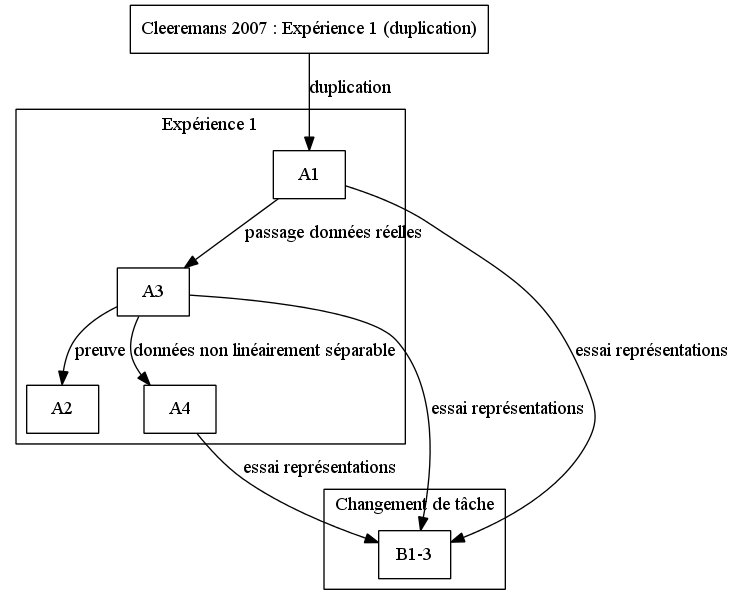
\includegraphics[height=320px]{data/workflow2.png}
  \end{center}
  
  \hspace*{-1.9cm}
  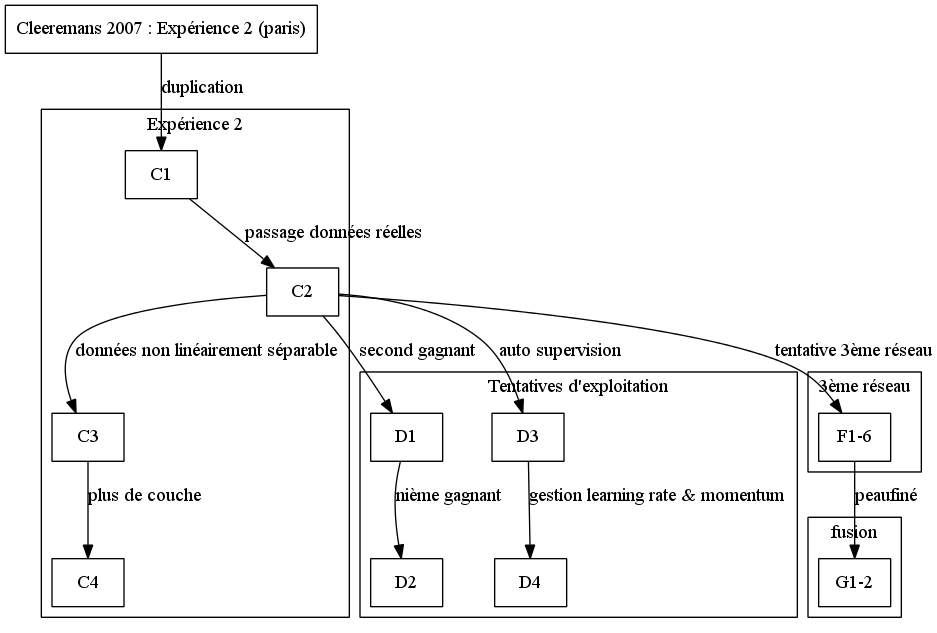
\includegraphics[width=550px]{data/workflow3.png}
  
  
  
  \section{Expérience A1} \label{expA1}
  \subsection{Objectif}
    Comprendre de quelles manières peuvent émerger des représentations et méta-représentations dans 
    un réseau de neurone connexionniste, plus particulièrement sur des perceptrons multicouches.
    
    
    Reproduction et approfondissement des résultats de la première expérience de l'article 
    \cite{Cleeremans_2007}. 

  \subsection{Architecture}
    \paragraph{Description}
      Un premier réseau de perceptron multicouche apprend à discrétiser des chiffres représentés
      par 20 neurones d'entrées. Il est composé d'une couche cachée de 5 neurones.
      
      Un second réseau de perceptron multicouche apprend à dupliquer toutes les couches du premier
      réseau en n'ayant que sa couche cachée en entrée.
      
      L'apprentissage du second réseau, n'affecte pas les poids entre la couche d'entrée et la 
      couche cachée du premier réseau.

    \paragraph{Schéma}
      \begin{center}
	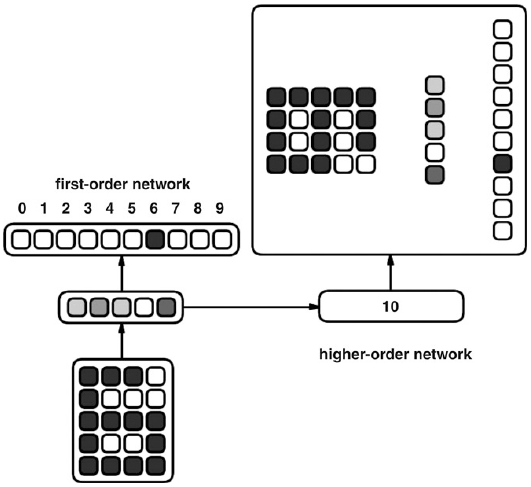
\includegraphics[width=220px]{data/expA1/schema.png}
      \end{center}
      
    \paragraph{Paramètres}
      \begin{center}
	\begin{tabular}{lr}
	  \begin{minipage}{220px}
	    \begin{itemize}
	      \item momentum : 0.9 sur les 2 réseau
	      \item taux d'apprentissage : 0.1 sur les 2 réseau
	      \item 10 chiffres différents présentés
	      \item apprentissage 10 (formes) x 1000 (époques)
	      \item utilisation de biais
	    \end{itemize}
	  \end{minipage}
	  &
	  \begin{minipage}{205px}
	    \begin{itemize}
	      \item poids initialisés sur [-0.25 ; 0.25]
	      \item taux d'apprentissage constant
	      \item entrées valent 0 ou 1
	      \item sigmoïde à température 1
	    \end{itemize}
	  \end{minipage}
	\end{tabular}
      \end{center}

  
  \newpage
  \subsection{Résultats}
    \paragraph{Principaux}
      Analyse des performances
      \begin{center}
	\begin{tabular}{lr}
	  \hspace*{-1cm}
	  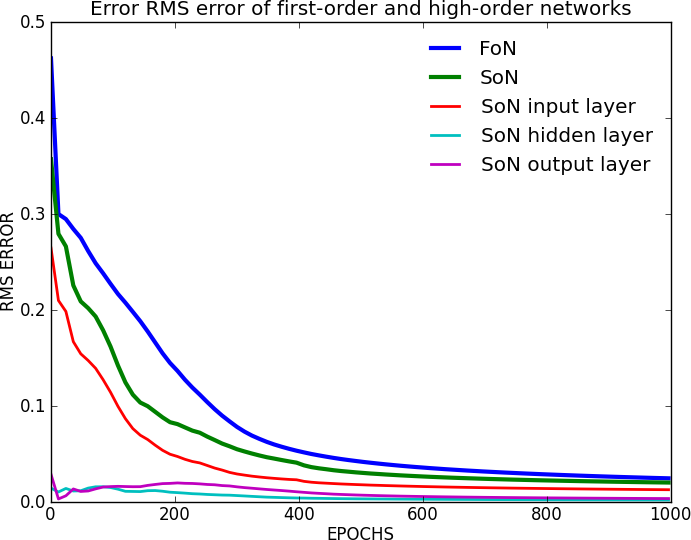
\includegraphics[width=250px]{data/expA1/rms.png}
	  &
	  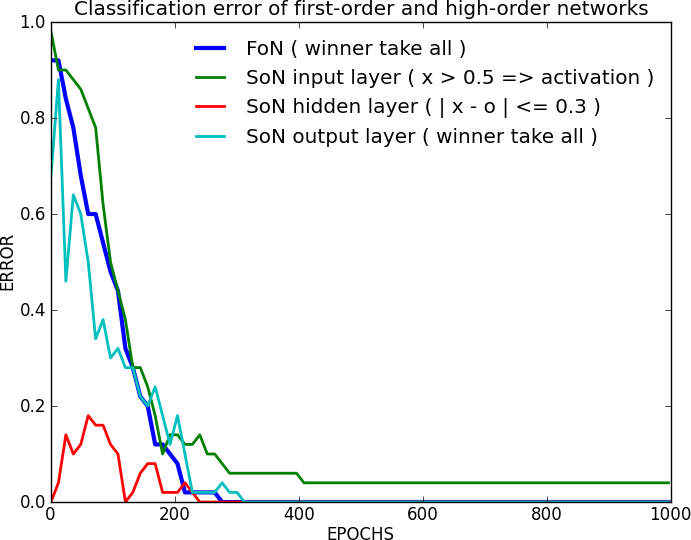
\includegraphics[width=250px]{data/expA1/err.png} 
	\end{tabular}
      \end{center}
      \subparagraph{Notes}
	\begin{itemize}
	  \item formule utilisée pour RMS (cf. Formules~\nameref{rms})
	  \item les courbes SoN layer représentent les erreurs (du second réseaux) sur les couches à reproduire 
	  \item la courbe RMS verte (SoN) est la somme des 3 courbes SoN layer
	\end{itemize}
      \subparagraph{Conclusion}
	\begin{itemize}
	  \item le premier réseau réussit à apprendre sa tâche de classification
	  \item la couche cachée et la couche de sortie ne posent aucun problèmes d'apprentissage
	  \item les performances du second réseau dépendent principalement de sa capacité à reproduire les entrées
	  \item le second réseau apprend plus rapidement que le premier
	\end{itemize}
    \paragraph{Secondaires}
      Discrétisation de la couche cachée du premier réseau
      \begin{center}
	\begin{tabular}{lr}
	  \hspace*{-1cm}
	  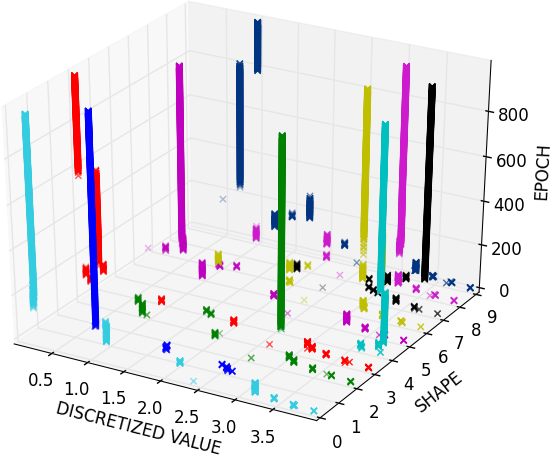
\includegraphics[width=250px]{data/expA1/discretize_cloud.png}
	  &
	  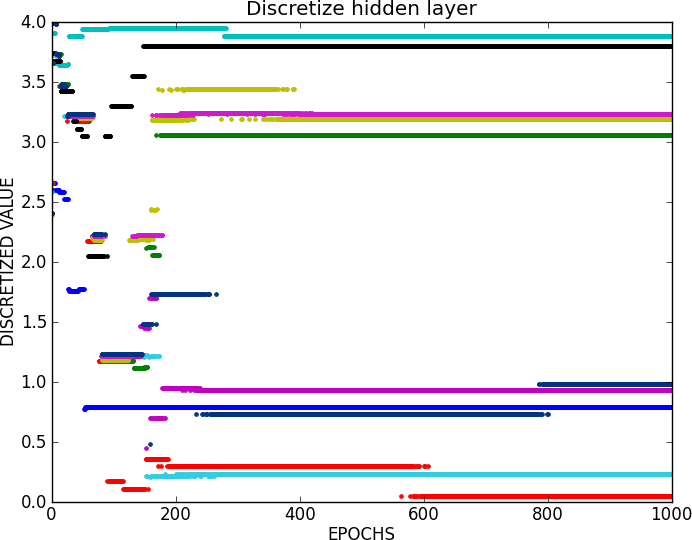
\includegraphics[width=250px]{data/expA1/discretize.png} 
	\end{tabular}
      \end{center} 
      \subparagraph{Notes}
	\begin{itemize}
	  \item une couleur équivaut à un chiffre présenté
	  \item une valeur discretisée correspond à un certain encodage de la couche cachée (cf Algorithmes~\nameref{discretize})
	\end{itemize}
      \subparagraph{Conclusion}
	Les neurones se stabilisent très rapidement (autour de la 50\up{ième} époque en moyenne), 
	le tout permettant au second réseau d'avoir des entrées très peu variables, favorisant
	son apprentissage.
    \paragraph{Secondaires}
      Représentations au travers des poids du premier réseau
      \begin{center}
	Couche cachée \\
	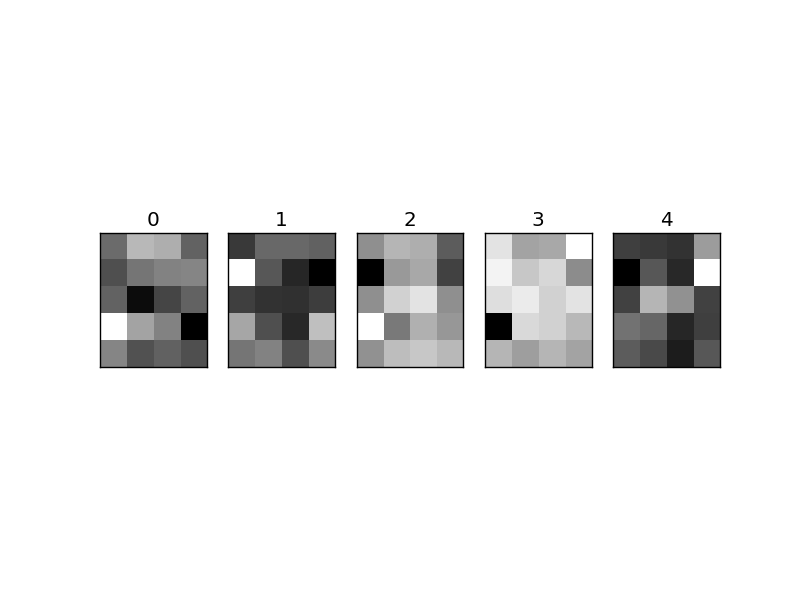
\includegraphics[width=250px]{data/expA1/representation_hidden.png}
      \end{center}
      \begin{center}
	Couche de sortie \\
	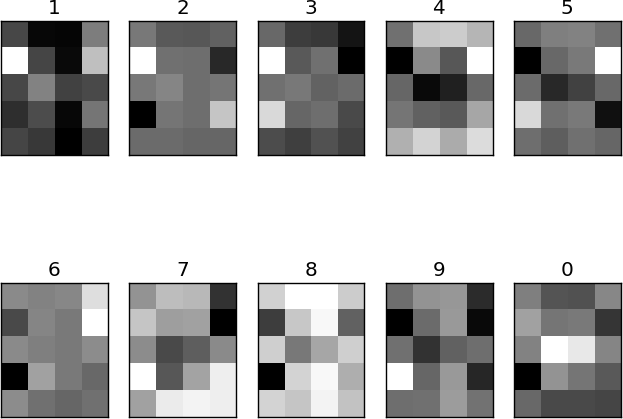
\includegraphics[width=250px]{data/expA1/representation.png}
      \end{center} 
      \subparagraph{Notes}
	\begin{itemize}
	  \item plus une case est noire, plus sa présence est importante pour le chiffre en question
	  \item plus une case est blanche, plus son absence est importante
	\end{itemize}
      \subparagraph{Conclusion}
	Il est assez difficile d'y distinquer les chiffres, mais cela semble suffisant pour le réseau
	qui a un taux de reconnaissance de 100\%.
    \paragraph{Secondaires}
      Prototypes à l'intérieur de la première partie de la couche de sortie du second réseau
      \begin{center}
	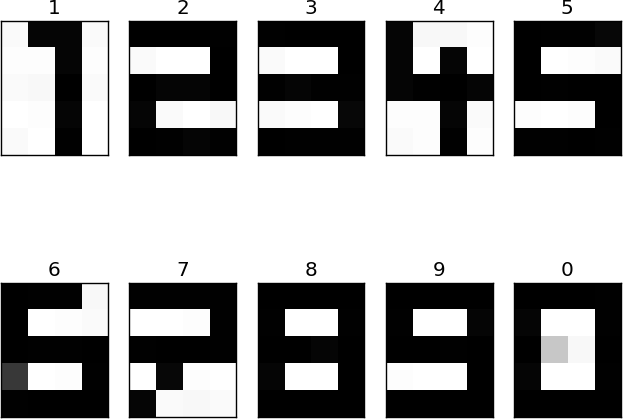
\includegraphics[width=250px]{data/expA1/prototype.png}
      \end{center} 
      \subparagraph{Notes}
	\begin{itemize}
	  \item Il sagit de la moyenne des réponses du second réseaux sur toutes les entrées
	\end{itemize}
      \subparagraph{Conclusion}
	Le peu d'entrées permet l'apprentissage par-coeur de chaque forme.
	


  \subsection{Conclusion}
  
  

  \newpage 
  \subsection{Formules}
    \paragraph{RMS} \label{rms}
  Pour une époque $e$ :
  \begin{center}
    \begin{large}
    $ rms_{e} = \sqrt{ \frac{1}{n} \sum \limits_{i=1}^{n} 
    ( o_{i,e} - d_{i} )^2 } $
    \end{large}
  $ with \left\lbrace \begin{array}{lll} n : number\ of\ neurons\ on\ the\ output\ 
  layer\\o_{i,e} : value\ obtained\ for\ the\ i^{th}\ neuron\ at\ the\ e^{th}\ epoch\\d_{i} : 
  value\ desired \ for\ the\ i^{th}\ neuron\end{array} \right.$
  \end{center}
    \paragraph{Discrétisation} \label{discretize}
      Pour la couche cachée $hiddenNeuron$ de $n$ neurones, un neurone
      pouvant être encodé par $number\_cutting$ valeurs différentes :
      \begin{center}
	$\sum \limits_{i=0}^{n} number\_cutting^{i} \times cutting(hiddenNeuron[i]) $
      \end{center}
      \subparagraph{Exemple}
	$400 \gets [0 ; 0,25 ]\ [0 ; 0,25 ]\  [0,25 ; 0,5 ]\  [0,5 ; 0,75 ]\  [0,25 ; 0,5 ]$ \\
	\hspace*{2.70cm}
	$400 \gets 0\times4^0 +   0\times4^1  +   1\times4^2   +  2\times4^3   +   1 \times4^4$
    \paragraph{Descente de gradient} \cite{Touzet_1992} \\
  Construction de l'erreur : 
    \begin{center}
      $y_{i} = f'(a_i) \times ( d_i - x_i ) \ si\ i\ neurone\ de\ sortie $ \\
      $y_{i} = f'(a_i) \times \sum \limits_{k} ( w_{ki} \times y_k )\ si\ i\ neurone\ cache $
    \end{center}
  Mise à jour des poids :
    \begin{center}
      $w_{ij}(t+1) = w_{ij}(t) + learning\_rate \times y_{i} \times x_j + momentum \times 
      (w_{ij}(t) - w_{ij}(t-1) )$
    \end{center}
  Variables : 
    \begin{center}
      $\left\lbrace \begin{array}{lll} 
	f : fonction\ sigmoide \\
	x_i : valeur\ du\ neurone\ i\\
	d_i : valeur\ desire pour\ le\ neurone\ i\\
	a_i : somme\ pondere\ des\ poids\ du\ neurone\ i
      \end{array} \right.$
    \end{center}
    
\bibliographystyle{../pre-rapport/apalike}
\bibliography{../pre-rapport/biblio}

  \section{Expérience A2} \label{expA2}
  \subsection{Objectif}
    Comprendre de quelles manières peuvent émerger des représentations et méta-représentations dans 
    un réseau de neurone connexionniste, plus particulièrement sur des perceptrons multicouches.
    
    Dans l'optique d'éprouver la première expérience de l'article \cite{Cleeremans_2007} sur des
    données plus réelles, il sagit, dans un premier temps, de montrer qu'une augmentation du 
    nombre de neurones, et qu'un simple agrandissement des chiffres en entrées, 
    n'affecte pas fondamentalement le fonctionnement du réseau.

  \subsection{Architecture}
    \paragraph{Description}
      Un premier réseau de perceptron multicouche apprend à discrétiser des chiffres représentés
      par 256 (16x16) neurones d'entrées. Il est composé d'une couche cachée de 64 neurones.
      
      Un second réseau de perceptron multicouche apprend à dupliquer toutes les couches du premier
      réseau en n'ayant que sa couche cachée en entrée.
      
      L'apprentissage du second réseau, n'affecte pas les poids entre la couche d'entrée et la 
      couche cachée du premier réseau.

    \paragraph{Schéma}
      \begin{center}
	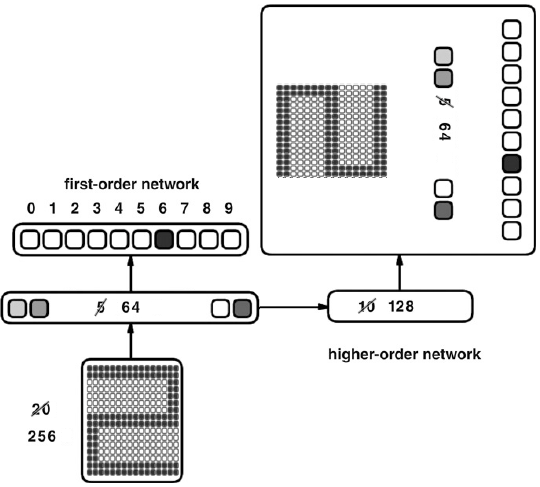
\includegraphics[width=220px]{data/expA2/schema.png}
      \end{center}
      
    \paragraph{Paramètres}
      \begin{center}
	\begin{tabular}{lr}
	  \begin{minipage}{230px}
	    \begin{itemize}
	      \item momentum : 0.9 sur les 2 réseaux
	      \item taux d'apprentissage : 0.1 sur les 2 réseaux
	      \item \textbf{10 formes} de chiffres différents présentées (shuffle)
	      \item apprentissage 10 (formes) x 1000 (époques)
	      \item utilisation de biais
	    \end{itemize}
	  \end{minipage}
	  &
	  \begin{minipage}{230px}
	    \begin{itemize}
	      \item poids initialisés sur [-0.25 ; 0.25]
	      \item taux d'apprentissage constant
	      \item entrées valent 0 ou 1
	      \item sigmoïde à température 1
	    \end{itemize}
	  \end{minipage}
	\end{tabular}
      \end{center}

  
  \newpage
  \subsection{Résultats}
    \paragraph{Principaux}
      Analyse des performances
      \begin{center}
	\begin{tabular}{lr}
	  \hspace*{-1cm}
	  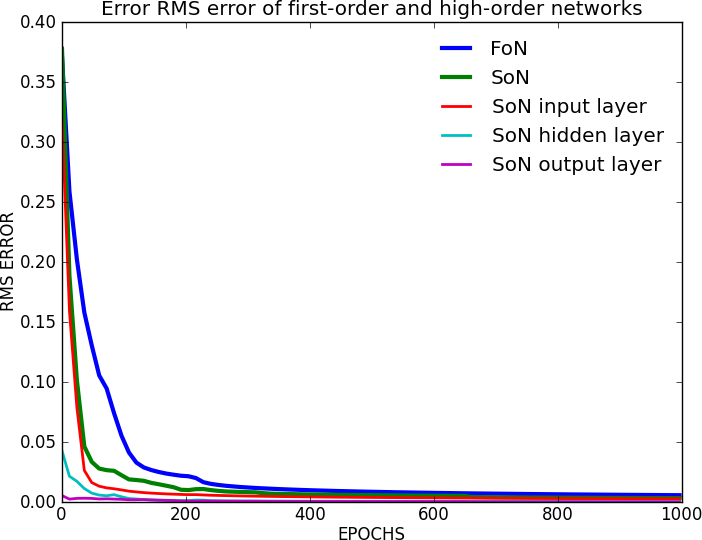
\includegraphics[width=250px]{data/expA2/rms.png}
	  &
	  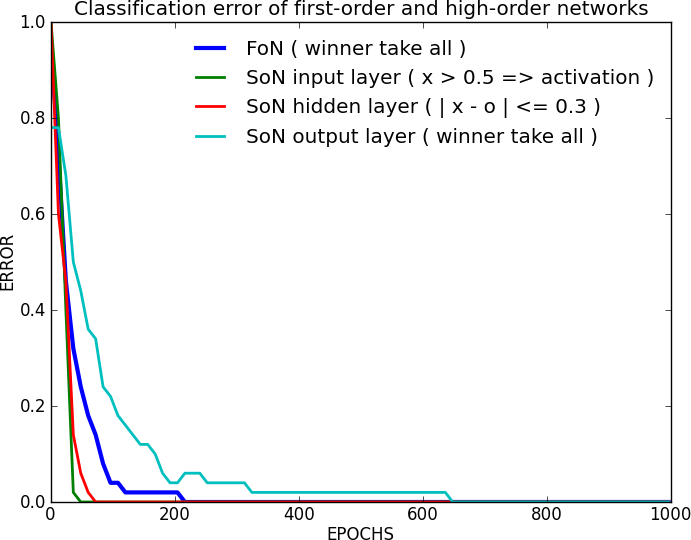
\includegraphics[width=250px]{data/expA2/err.png} 
	\end{tabular}
      \end{center}
      \subparagraph{Notes}
	\begin{itemize}
	  \item formule utilisée pour RMS (cf. Formules~\nameref{rms})
	  \item les courbes SoN layer représentent les erreurs (du second réseaux) sur les couches à reproduire 
	  \item la courbe RMS verte (SoN) est la somme des 3 courbes SoN layer
	\end{itemize}
      \subparagraph{Conclusion}
	\begin{itemize}
	  \item le premier réseau réussit à apprendre sa tâche de classification
	  \item la couche cachée et la couche de sortie ne posent aucun problèmes d'apprentissage
	  \item les performances du second réseau dépendent principalement de sa capacité à reproduire les entrées
	  \item le second réseau apprend plus rapidement que le premier
	  \item l'augmentation du nombre de neurone ne change pas les tendances des courbes
	\end{itemize}
    \paragraph{Secondaires}
      Discrétisation de la couche cachée du premier réseau
      \begin{center}
	\begin{tabular}{lr}
	  \hspace*{-1cm}
	  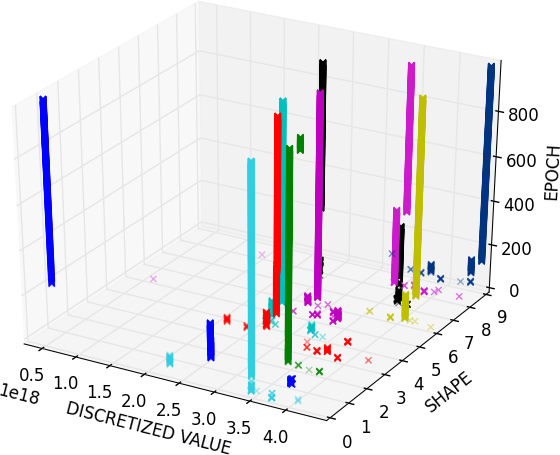
\includegraphics[width=250px]{data/expA2/discretize_cloud.png}
	  &
	  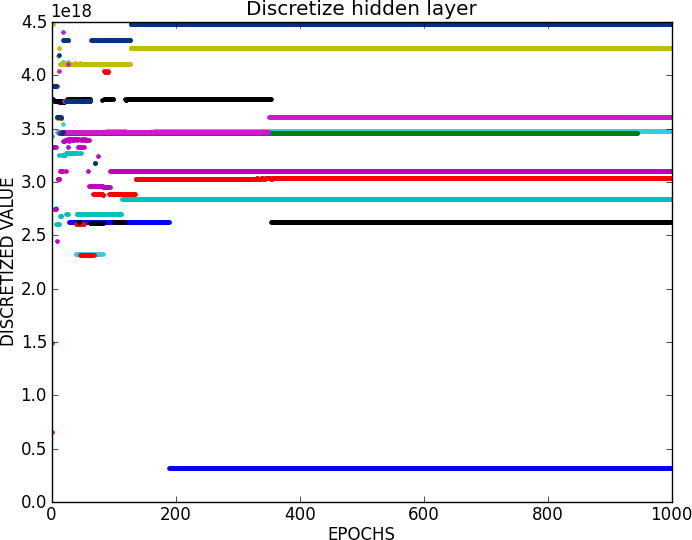
\includegraphics[width=250px]{data/expA2/discretize.png} 
	\end{tabular}
      \end{center} 
      \subparagraph{Notes}
	\begin{itemize}
	  \item une couleur équivaut à un chiffre présenté
	  \item une valeur discretisée correspond à un certain encodage de la couche cachée (cf Algorithmes~\nameref{discretize})
	\end{itemize}
      \subparagraph{Conclusion}
	Les neurones se stabilisent très rapidement (autour de la 50\up{ième} époque en moyenne), 
	le tout permettant au second réseau d'avoir des entrées très peu variables, favorisant
	son apprentissage.
    \paragraph{Secondaires}
      Représentations au travers des poids du premier réseau
      \begin{center}
	Couche cachée \\
	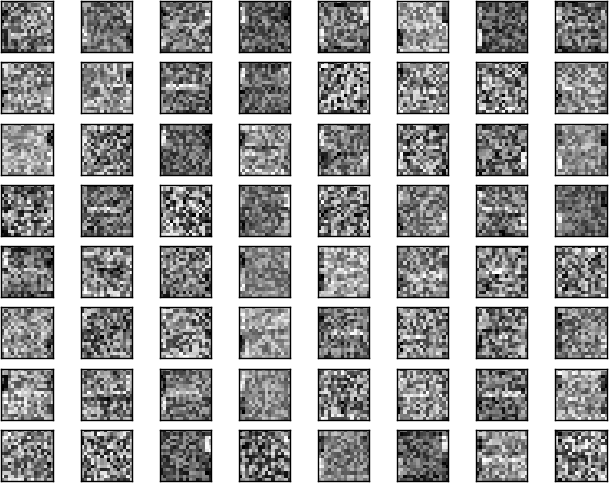
\includegraphics[width=250px]{data/expA2/representation_hidden.png}
      \end{center}
      \begin{center}
	Couche de sortie \\
	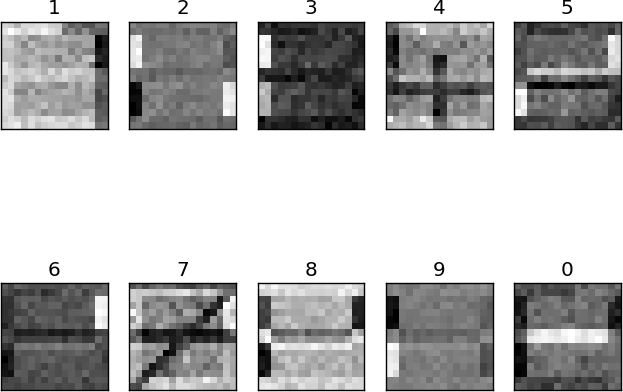
\includegraphics[width=250px]{data/expA2/representation.png}
      \end{center} 
      \subparagraph{Notes}
	\begin{itemize}
	  \item plus une case est noire, plus sa présence est importante pour le chiffre en question
	  \item plus une case est blanche, plus son absence est importante
	\end{itemize}
      \subparagraph{Conclusion}
      Il est intéréssant de remarquer qu'au vu du peu d'entrée, le réseau cible des neurones très précis.
      Pour le chiffre 2, par exemple, seul 3 lignes sont ciblées.
    \paragraph{Secondaires}
      Prototypes à l'intérieur de la première partie de la couche de sortie du second réseau
      \begin{center}
	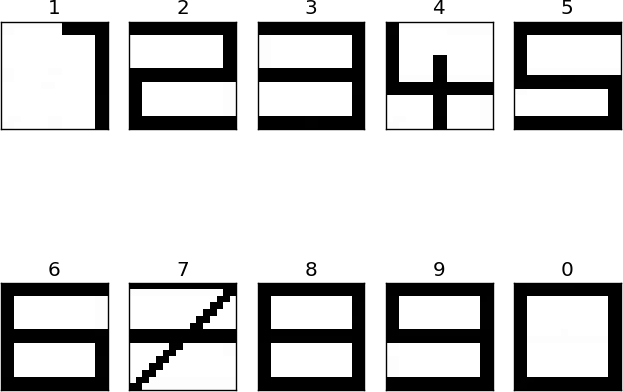
\includegraphics[width=250px]{data/expA2/prototype.png}
      \end{center} 
      \subparagraph{Notes}
	\begin{itemize}
	  \item Il sagit de la moyenne des réponses du second réseaux sur toutes les entrées
	\end{itemize}
      \subparagraph{Conclusion}
	Le peu d'entrées permet l'apprentissage par-coeur de chaque forme.
	


  \subsection{Conclusion}
    L'augmentation du nombre de neurones dans le réseau, et l'augmentation de la taille des entrées
    ne modifient pas l'attitude du réseau.
  

  \newpage 
  \subsection{Formules}
    \paragraph{RMS} \label{rms}
  Pour une époque $e$ :
  \begin{center}
    \begin{large}
    $ rms_{e} = \sqrt{ \frac{1}{n} \sum \limits_{i=1}^{n} 
    ( o_{i,e} - d_{i} )^2 } $
    \end{large}
  $ with \left\lbrace \begin{array}{lll} n : number\ of\ neurons\ on\ the\ output\ 
  layer\\o_{i,e} : value\ obtained\ for\ the\ i^{th}\ neuron\ at\ the\ e^{th}\ epoch\\d_{i} : 
  value\ desired \ for\ the\ i^{th}\ neuron\end{array} \right.$
  \end{center}
    \paragraph{Discrétisation} \label{discretize}
      Pour la couche cachée $hiddenNeuron$ de $n$ neurones, un neurone
      pouvant être encodé par $number\_cutting$ valeurs différentes :
      \begin{center}
	$\sum \limits_{i=0}^{n} number\_cutting^{i} \times cutting(hiddenNeuron[i]) $
      \end{center}
      \subparagraph{Exemple}
	$400 \gets [0 ; 0,25 ]\ [0 ; 0,25 ]\  [0,25 ; 0,5 ]\  [0,5 ; 0,75 ]\  [0,25 ; 0,5 ]$ \\
	\hspace*{2.70cm}
	$400 \gets 0\times4^0 +   0\times4^1  +   1\times4^2   +  2\times4^3   +   1 \times4^4$
    \paragraph{Descente de gradient} \cite{Touzet_1992} \\
  Construction de l'erreur : 
    \begin{center}
      $y_{i} = f'(a_i) \times ( d_i - x_i ) \ si\ i\ neurone\ de\ sortie $ \\
      $y_{i} = f'(a_i) \times \sum \limits_{k} ( w_{ki} \times y_k )\ si\ i\ neurone\ cache $
    \end{center}
  Mise à jour des poids :
    \begin{center}
      $w_{ij}(t+1) = w_{ij}(t) + learning\_rate \times y_{i} \times x_j + momentum \times 
      (w_{ij}(t) - w_{ij}(t-1) )$
    \end{center}
  Variables : 
    \begin{center}
      $\left\lbrace \begin{array}{lll} 
	f : fonction\ sigmoide \\
	x_i : valeur\ du\ neurone\ i\\
	d_i : valeur\ desire pour\ le\ neurone\ i\\
	a_i : somme\ pondere\ des\ poids\ du\ neurone\ i
      \end{array} \right.$
    \end{center}

\bibliographystyle{../pre-rapport/apalike}
\bibliography{../pre-rapport/biblio}

  \section{Expérience A3} \label{expA3}
  \subsection{Objectif}
    Comprendre de quelles manières peuvent émerger des représentations et méta-représentations dans 
    un réseau de neurone connexionniste, plus particulièrement sur des perceptrons multicouches.
    
    Réalisation de la première expérience de l'article \cite{Cleeremans_2007} sur des données réelles.
    
  \subsection{Architecture}
    \paragraph{Description}
      Un premier réseau de perceptron multicouche apprend à discrétiser des chiffres représentés
      par 256 (16x16) neurones d'entrées. Il est composé d'une couche cachée de 64 neurones.
      
      Un second réseau de perceptron multicouche apprend à dupliquer toutes les couches du premier
      réseau en n'ayant que sa couche cachée en entrée.
      
      L'apprentissage du second réseau, n'affecte pas les poids entre la couche d'entrée et la 
      couche cachée du premier réseau.

    \paragraph{Schéma}
      \begin{center}
	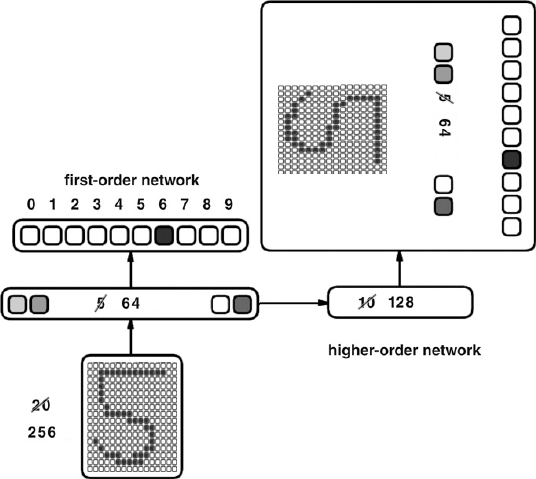
\includegraphics[width=220px]{data/expA3/schema.png}
      \end{center}
      
    \paragraph{Paramètres}
      \begin{center}
	\begin{tabular}{lr}
	  \begin{minipage}{230px}
	    \begin{itemize}
	      \item momentum : 0.9 sur les 2 réseaux
	      \item taux d'apprentissage : 0.1 sur les 2 réseaux
	      \item \textbf{1600 formes} de chiffres différents présentées (shuffle) \cite{Handwritten_256}
	      \item apprentissage 10 (formes) x 1000 (époques)
	    \end{itemize}
	  \end{minipage}
	  &
	  \begin{minipage}{230px}
	    \begin{itemize}
	      \item poids initialisés sur [-0.25 ; 0.25]
	      \item taux d'apprentissage constant
	      \item entrées valent 0 ou 1
	      \item sigmoïde à température 1
	      \item utilisation de biais
	    \end{itemize}
	  \end{minipage}
	\end{tabular}
      \end{center}

  
  \newpage
  \subsection{Résultats}
    \paragraph{Principaux}
      Analyse des performances
      \begin{center}
	\begin{tabular}{lr}
	  \hspace*{-1cm}
	  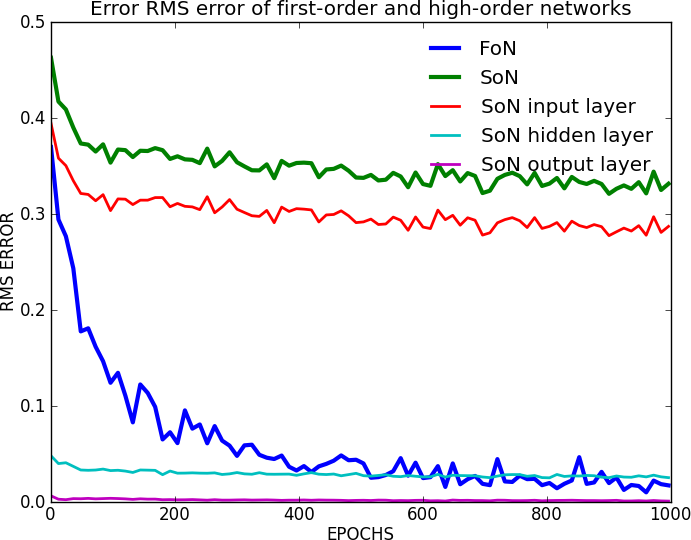
\includegraphics[width=250px]{data/expA3/rms.png}
	  &
	  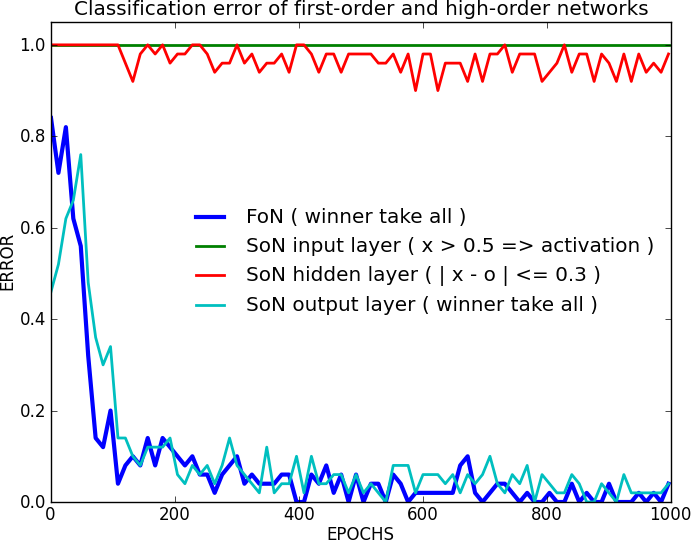
\includegraphics[width=250px]{data/expA3/err.png} 
	\end{tabular}
      \end{center}
      \subparagraph{Notes}
	\begin{itemize}
	  \item formule utilisée pour RMS (cf. Formules~\nameref{rms})
	  \item les courbes SoN layer représentent les erreurs (du second réseaux) sur les couches à reproduire 
	  \item la courbe RMS verte (SoN) est la somme des 3 courbes SoN layer
	  \item l'erreur de classification représente le taux de mauvaises réponses pour les 10 formes présentées sur une époque
	  \item pour SoN input layer et hidden layer, un winner-take-all n'est pas possible (ce n'est pas de la classification, 
	  mais une duplication), il y a donc un seuil d'erreur qui ne doit pas être dépassé par un seul neurone
	\end{itemize}
      \subparagraph{Conclusion}
	\begin{itemize}
	  \item le premier réseau réussit à apprendre sa tâche de classification
	  \item le second réseau \textbf{ne réussit pas} à apprendre sa tâche de duplication ( seul la couche cachée et de sortie sont apprisent )
	  \item la couche cachée et la couche de sortie posent peu de problèmes d'apprentissage
	  \item le second réseau a du mal à reproduire les entrées
	  \item le second réseau apprend maintenant (vs \nameref{expA1}, \nameref{expA2}) moins rapidement que le premier
	\end{itemize}
	
    \paragraph{Secondaires}
      RMS indépendant par couche
      \begin{center}
	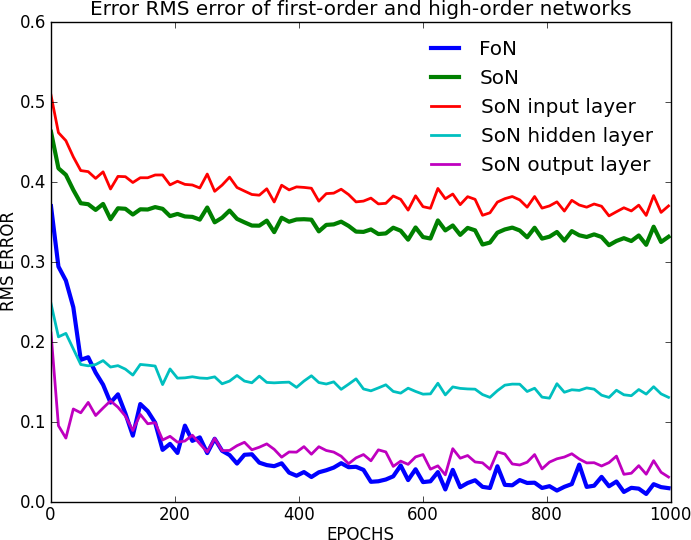
\includegraphics[width=250px]{data/expA3/rms_new.png}
      \end{center}
      \subparagraph{Notes}
	\begin{itemize}
	  \item formule utilisée pour RMS (cf. Formules~\nameref{rms})
	  \item les courbes SoN layer représentent les erreurs (du second réseaux) sur les couches à reproduire
	  \item les erreurs de SoN sont calculées en divisant par le nombre de neurone de la couche à reproduire (et non par le nombre total de neurones)
	\end{itemize}
      \subparagraph{Conclusion}
	\begin{itemize}
	  \item le SoN a plus de mal à apprendre la couche cachée que celle de sortie
	\end{itemize}
	
	
    \paragraph{Secondaires}
      Discrétisation de la couche cachée du premier réseau
      \begin{center}
	\begin{tabular}{lr}
	  \hspace*{-1cm}
	  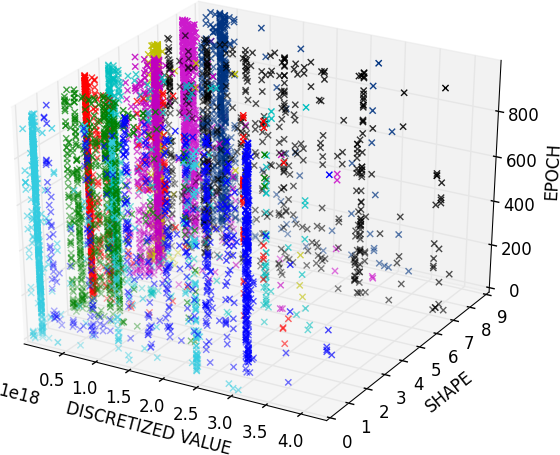
\includegraphics[width=250px]{data/expA3/discretize_cloud.png}
	  &
	  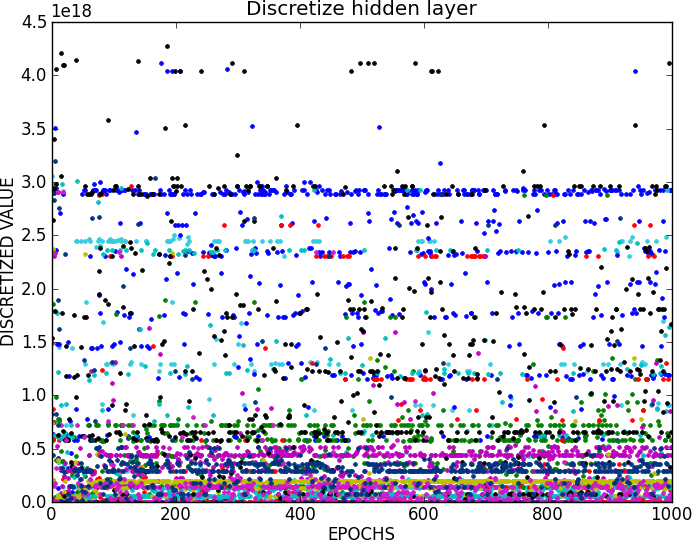
\includegraphics[width=250px]{data/expA3/discretize.png} 
	\end{tabular}
      \end{center} 
      \subparagraph{Notes}
	\begin{itemize}
	  \item une couleur équivaut à un chiffre présenté
	  \item une valeur discretisée correspond à un certain encodage de la couche cachée (cf Algorithmes~\nameref{discretize})
	\end{itemize}
      \subparagraph{Conclusion}
	Nous pouvons maintenant expliquer les raisons provoquant le mauvais apprentissage des entrées par le second réseau :
	
	Pour un seul chiffre présenté, il existe différentes valeurs de la couche cachée le représentant ( factorisation 
	dans la couche cachée du premier réseau). Le second réseau ne peut donc pas apprendre toutes les entrées.
	
	Une même valeur discretisée peut correspondre à plusieurs couleurs (différents nombres) ce qui augmentent la 
	difficulté d'apprentissage.
    \paragraph{Secondaires}
      Représentations au travers des poids du premier réseau
      \begin{center}
	Couche cachée \\
	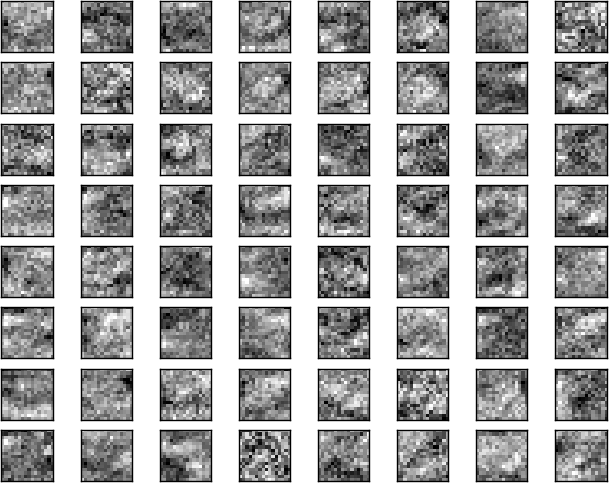
\includegraphics[width=250px]{data/expA3/representation_hidden.png}
      \end{center}
      \begin{center}
	Couche de sortie \\
	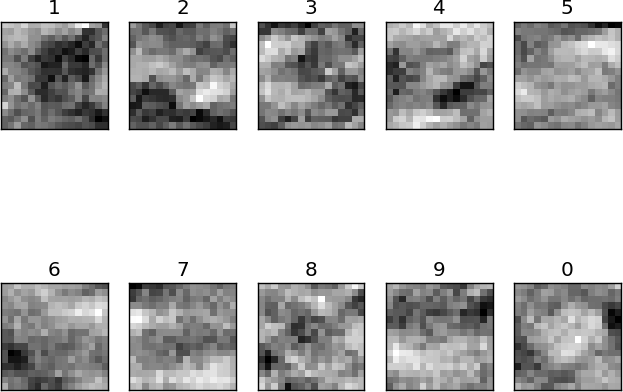
\includegraphics[width=250px]{data/expA3/representation.png}
      \end{center} 
      \subparagraph{Notes}
	\begin{itemize}
	  \item plus une case est noire, plus sa présence est importante pour le chiffre en question
	  \item plus une case est blanche, plus son absence est importante
	  \item c'est seulement lorsqu'elle est grise qu'elle n'est pas prise en compte
	\end{itemize}
      \subparagraph{Conclusion}
	On arrive, sans trop de mal, à distinguer les chiffres.
    \paragraph{Secondaires}
      Prototypes à l'intérieur des neurones du second réseau qui essaient de redonner les entrées
      \begin{center}
	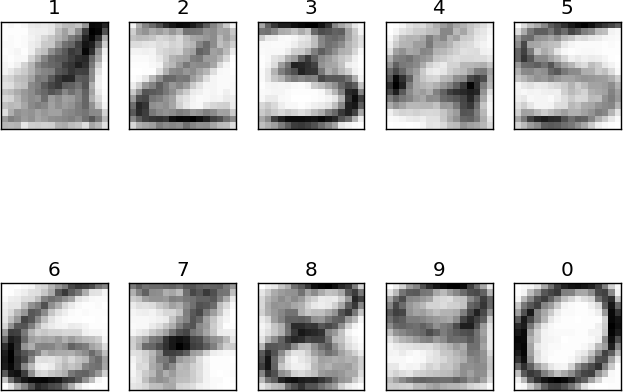
\includegraphics[width=250px]{data/expA3/prototype.png}
      \end{center} 
      \subparagraph{Notes}
	\begin{itemize}
	  \item Il sagit de la moyenne des réponses du second réseaux sur toutes les entrées
	\end{itemize}
      \subparagraph{Conclusion}
	Il est intéressant de constaté que malgrès la difficulté de la tâche, ces prototypes émergent.
	
	Et que contrairement à ce qu'indique les performances, les chiffres sont bien distincts.
      
	On peut, par ailleurs, conjecturer que plus la couche cachée du premier réseau est petite, plus les prototypes 
	seront factorisés (ie. personnels au réseau).
	


  \subsection{Conclusion}
    Comme il l'est dit dans \cite{Cleeremans_2007}, cette architecture tente de résoudre les problèmes des réseaux connexionnistes
  classiques à avoir un semblant de conscience.
  
  À savoir :
  \begin{itemize}
   \item qu'ils ne savent pas qu'ils peuvent se trouver dans différents états, et qu'ils ne traitent pas leurs propres états : 
   d'où la présence de ce second réseau qui tente de traiter ses états et d'apprendre qu'il en a plusieurs
   \item des représentations rentant bloquées dans la chaîne de causalité de la tâche à apprendre : d'où
   le fait que ce second réseau n'affecte pas l'apprentissage du premier (ie. pour ne pas retomber dans la chaîne de causalité)
   \\[0.2cm]
  \end{itemize}
  
  Lors de l'\nameref{expA4}, nous avons confronter la même architecture à des données non linéairement séparables.
  
  Dans l'\nameref{expB2}, nous avons expérimenté les représentations et le transfert de tâche.
  

  \newpage 
  \subsection{Formules}
    \paragraph{RMS} \label{rms}
  Pour une époque $e$ :
  \begin{center}
    \begin{large}
    $ rms_{e} = \sqrt{ \frac{1}{n} \sum \limits_{i=1}^{n} 
    ( o_{i,e} - d_{i} )^2 } $
    \end{large}
  $ with \left\lbrace \begin{array}{lll} n : number\ of\ neurons\ on\ the\ output\ 
  layer\\o_{i,e} : value\ obtained\ for\ the\ i^{th}\ neuron\ at\ the\ e^{th}\ epoch\\d_{i} : 
  value\ desired \ for\ the\ i^{th}\ neuron\end{array} \right.$
  \end{center}
    \paragraph{Discrétisation} \label{discretize}
      Pour la couche cachée $hiddenNeuron$ de $n$ neurones, un neurone
      pouvant être encodé par $number\_cutting$ valeurs différentes :
      \begin{center}
	$\sum \limits_{i=0}^{n} number\_cutting^{i} \times cutting(hiddenNeuron[i]) $
      \end{center}
      \subparagraph{Exemple}
	$400 \gets [0 ; 0,25 ]\ [0 ; 0,25 ]\  [0,25 ; 0,5 ]\  [0,5 ; 0,75 ]\  [0,25 ; 0,5 ]$ \\
	\hspace*{2.70cm}
	$400 \gets 0\times4^0 +   0\times4^1  +   1\times4^2   +  2\times4^3   +   1 \times4^4$
    \paragraph{Descente de gradient} \cite{Touzet_1992} \\
  Construction de l'erreur : 
    \begin{center}
      $y_{i} = f'(a_i) \times ( d_i - x_i ) \ si\ i\ neurone\ de\ sortie $ \\
      $y_{i} = f'(a_i) \times \sum \limits_{k} ( w_{ki} \times y_k )\ si\ i\ neurone\ cache $
    \end{center}
  Mise à jour des poids :
    \begin{center}
      $w_{ij}(t+1) = w_{ij}(t) + learning\_rate \times y_{i} \times x_j + momentum \times 
      (w_{ij}(t) - w_{ij}(t-1) )$
    \end{center}
  Variables : 
    \begin{center}
      $\left\lbrace \begin{array}{lll} 
	f : fonction\ sigmoide \\
	x_i : valeur\ du\ neurone\ i\\
	d_i : valeur\ desire pour\ le\ neurone\ i\\
	a_i : somme\ pondere\ des\ poids\ du\ neurone\ i
      \end{array} \right.$
    \end{center}

\bibliographystyle{../pre-rapport/apalike}
\bibliography{../pre-rapport/biblio}

  \section{Expérience A4} \label{expA4}
  \subsection{Objectif}
    Comprendre de quelles manières peuvent émerger des représentations et méta-représentations dans 
    un réseau de neurone connexionniste, plus particulièrement sur des perceptrons multicouches.
    
    Réalisation de la première expérience de l'article \cite{Cleeremans_2007} sur des données réelles
    et non linéairement séparables.

  
  \subsection{Architecture}
    \paragraph{Description}
      Un premier réseau de perceptron multicouche apprend à discrétiser des fleurs caractérisées
      par 4 neurones d'entrées qui représentent taille et largeur de la pétale et la sépale. 
      Il est composé d'une couche cachée de 5 neurones.
      
      Un second réseau de perceptron multicouche apprend à dupliquer toutes les couches du premier
      réseau en n'ayant que sa couche cachée en entrée.
      
      L'apprentissage du second réseau, n'affecte pas les poids entre la couche d'entrée et la 
      couche cachée du premier réseau.

    \paragraph{Schéma}
      \begin{center}
	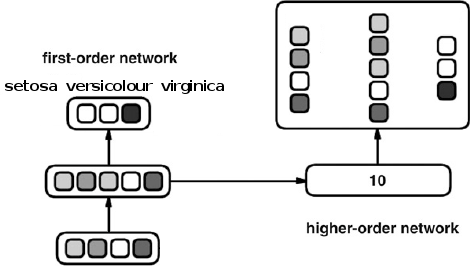
\includegraphics[width=230px]{data/expA4/schema.png}
      \end{center}
      
    \paragraph{Paramètres}
      \begin{center}
	\begin{tabular}{lr}
	  \begin{minipage}{230px}
	    \begin{itemize}
	      \item momentum : 0.9 sur les 2 réseaux
	      \item taux d'apprentissage : 0.1 sur les 2 réseaux
	      \item 150 fleurs différentes présentés \cite{Iris}
	      \item apprentissage 10 (formes) x 1000 (époques)
	      \item utilisation de biais
	    \end{itemize}
	  \end{minipage}
	  &
	  \begin{minipage}{230px}
	    \begin{itemize}
	      \item poids initialisés sur [-0.25 ; 0.25]
	      \item taux d'apprentissage constant
	      \item entrées réelles sur [0 ; 1]
	      \item sigmoïde à température 1
	    \end{itemize}
	  \end{minipage}
	\end{tabular}
      \end{center}

  
  \newpage
  \subsection{Résultats}
    \paragraph{Principaux}
      Analyse des performances
      \begin{center}
	\begin{tabular}{lr}
	  \hspace*{-1cm}
	  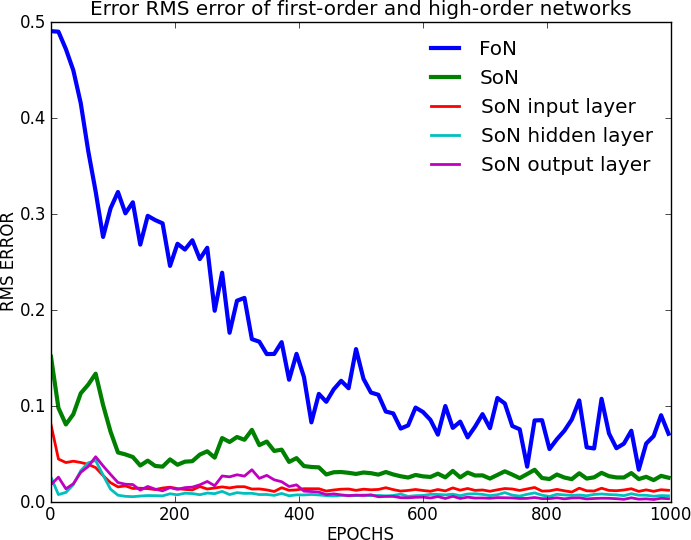
\includegraphics[width=250px]{data/expA4/rms.png}
	  &
	  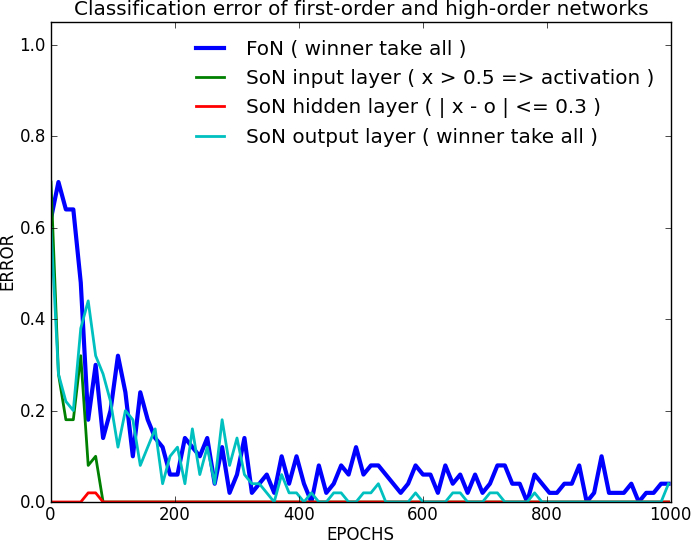
\includegraphics[width=250px]{data/expA4/err.png} 
	\end{tabular}
      \end{center}
      \subparagraph{Notes}
	\begin{itemize}
	  \item formule utilisée pour RMS (cf. Formules~\nameref{rms})
	  \item les courbes SoN layer représentent les erreurs (du second réseaux) sur les couches à reproduire 
	  \item la courbe RMS verte (SoN) est la somme des 3 courbes SoN layer
	  \item l'erreur de classification représente le taux de mauvaises réponses pour les 10 formes présentées sur une époque
	  \item pour SoN input layer et hidden layer, un winner-take-all n'est pas possible (ce n'est pas de la classification, 
	  mais une duplication), il y a donc un seuil d'erreur qui ne doit pas être dépassé par un seul neurone
	\end{itemize}
      \subparagraph{Conclusion}
	\begin{itemize}
	  \item le premier réseau réussit à apprendre sa tâche de classification
	  \item le second réseau réussit à apprendre sa tâche de duplication
	  \item la couche cachée et la couche de sortie posent peu de problèmes d'apprentissage
	  \item les performances du second réseau dépendent principalement de sa capacité à reproduire les entrées
	  \item le second réseau apprend plus rapidement que le premier
	\end{itemize}

    \paragraph{Secondaires}
      RMS indépendant par couche
      \begin{center}
	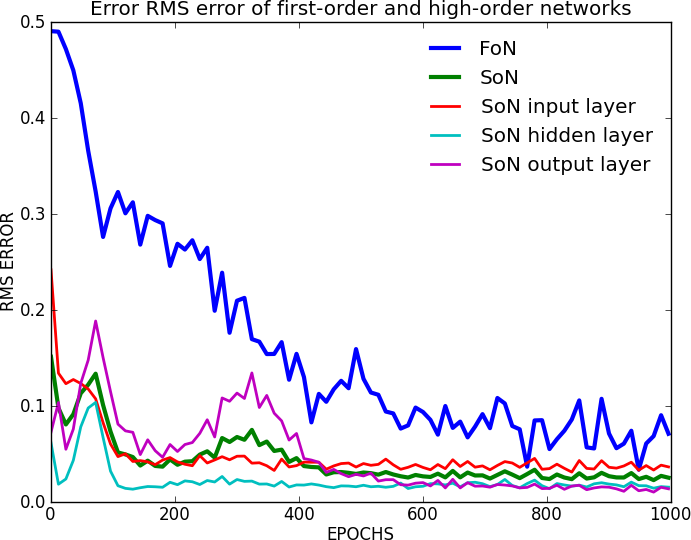
\includegraphics[width=250px]{data/expA4/rms_new.png}
      \end{center}
      \subparagraph{Notes}
	\begin{itemize}
	  \item formule utilisée pour RMS (cf. Formules~\nameref{rms})
	  \item les courbes SoN layer représentent les erreurs (du second réseaux) sur les couches à reproduire
	  \item les erreurs de SoN sont calculées en divisant par le nombre de neurone de la couche à reproduire (et non par le nombre total de neurones)
	\end{itemize}
      \subparagraph{Conclusion}
	

    \paragraph{Secondaires}
      Discrétisation de la couche cachée du premier réseau
      \begin{center}
	\begin{tabular}{lr}
	  \hspace*{-1cm}
	  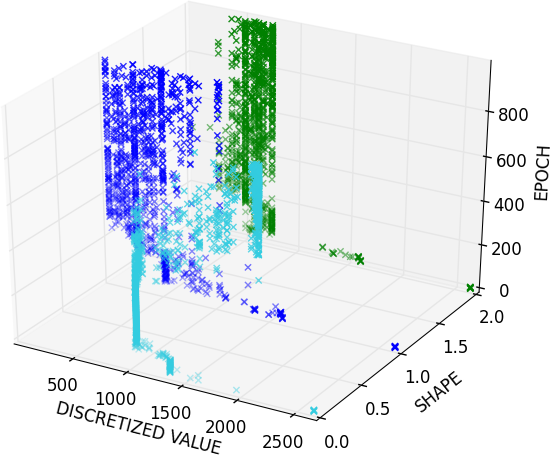
\includegraphics[width=250px]{data/expA4/discretize_cloud.png}
	  &
	  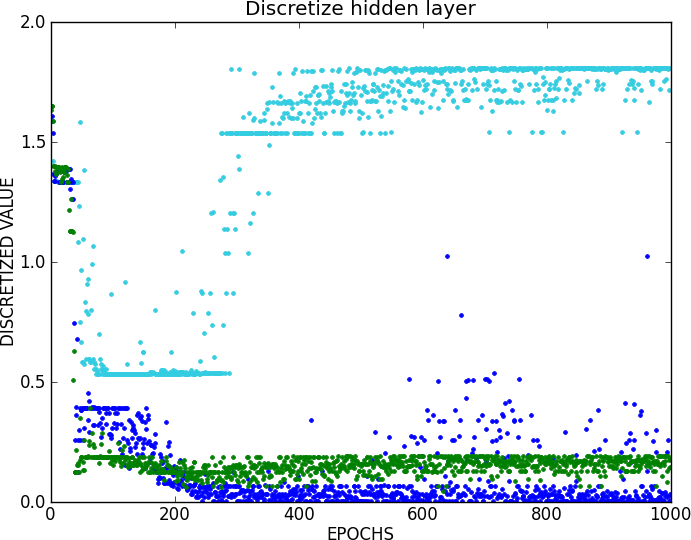
\includegraphics[width=250px]{data/expA4/discretize.png} 
	\end{tabular}
      \end{center} 
      \subparagraph{Notes}
	\begin{itemize}
	  \item une couleur équivaut à une fleur présentée
	  \item une valeur discretisée correspond à un certain encodage de la couche cachée (cf Algorithmes~\nameref{discretize})
	\end{itemize}
      \subparagraph{Conclusion}
	Les données n'étant pas linéairement séparables, leur passage dans une seule couche rend la tâche d'apprentissage
	du second réseau plus complexe.
	
	On peut voir plusieurs points de différentes couleurs aux mêmes endroits (ie. pour la même couche cachée).

  \subsection{Conclusion}
  Le passage sur des données non linéairement séparables se passent bien.
  
  Comme il l'est dit dans \cite{Cleeremans_2007}, cette architecture tente de résoudre les problèmes des réseaux connexionnistes
  classiques à avoir un semblant de conscience.
  
  À savoir :
  \begin{itemize}
   \item qu'ils ne savent pas qu'ils peuvent se trouver dans différents états, et qu'ils ne traitent pas leurs propres états : 
   d'où la présence de ce second réseau qui tente de traiter ses états et d'apprendre qu'il en a plusieurs
   \item des représentations rentant bloquées dans la chaîne de causalité de la tâche à apprendre : d'où
   le fait que ce second réseau n'affecte pas l'apprentissage du premier (ie. pour ne pas retomber dans la chaîne de causalité)
   \\[0.2cm]
  \end{itemize}
  
  Dans l'\nameref{expB3}, nous avons expérimenté les représentations et le transfert de tâche.
  

  \newpage 
  \subsection{Formules}
    \paragraph{RMS} \label{rms}
  Pour une époque $e$ :
  \begin{center}
    \begin{large}
    $ rms_{e} = \sqrt{ \frac{1}{n} \sum \limits_{i=1}^{n} 
    ( o_{i,e} - d_{i} )^2 } $
    \end{large}
  $ with \left\lbrace \begin{array}{lll} n : number\ of\ neurons\ on\ the\ output\ 
  layer\\o_{i,e} : value\ obtained\ for\ the\ i^{th}\ neuron\ at\ the\ e^{th}\ epoch\\d_{i} : 
  value\ desired \ for\ the\ i^{th}\ neuron\end{array} \right.$
  \end{center}
    \paragraph{Discrétisation} \label{discretize}
      Pour la couche cachée $hiddenNeuron$ de $n$ neurones, un neurone
      pouvant être encodé par $number\_cutting$ valeurs différentes :
      \begin{center}
	$\sum \limits_{i=0}^{n} number\_cutting^{i} \times cutting(hiddenNeuron[i]) $
      \end{center}
      \subparagraph{Exemple}
	$400 \gets [0 ; 0,25 ]\ [0 ; 0,25 ]\  [0,25 ; 0,5 ]\  [0,5 ; 0,75 ]\  [0,25 ; 0,5 ]$ \\
	\hspace*{2.70cm}
	$400 \gets 0\times4^0 +   0\times4^1  +   1\times4^2   +  2\times4^3   +   1 \times4^4$
    \paragraph{Descente de gradient} \cite{Touzet_1992} \\
  Construction de l'erreur : 
    \begin{center}
      $y_{i} = f'(a_i) \times ( d_i - x_i ) \ si\ i\ neurone\ de\ sortie $ \\
      $y_{i} = f'(a_i) \times \sum \limits_{k} ( w_{ki} \times y_k )\ si\ i\ neurone\ cache $
    \end{center}
  Mise à jour des poids :
    \begin{center}
      $w_{ij}(t+1) = w_{ij}(t) + learning\_rate \times y_{i} \times x_j + momentum \times 
      (w_{ij}(t) - w_{ij}(t-1) )$
    \end{center}
  Variables : 
    \begin{center}
      $\left\lbrace \begin{array}{lll} 
	f : fonction\ sigmoide \\
	x_i : valeur\ du\ neurone\ i\\
	d_i : valeur\ desire pour\ le\ neurone\ i\\
	a_i : somme\ pondere\ des\ poids\ du\ neurone\ i
      \end{array} \right.$
    \end{center}

\bibliographystyle{../pre-rapport/apalike}
\bibliography{../pre-rapport/biblio}

  \section{Expérience B1} \label{expB1}
  \subsection{Objectif}
    Comprendre de quelles manières peuvent émerger des représentations et méta-représentations dans 
    un réseau de neurone connexionniste, plus particulièrement sur des perceptrons multicouches.
    
    
    À partir de la première expérience de l'article \cite{Cleeremans_2007}, expérimenter les représentations.
  
  \subsection{Architecture}
    \paragraph{Description}
      Un premier réseau de perceptron multicouche apprend à discrétiser des chiffres représentés
      par 20 neurones d'entrées. Il est composé d'une couche cachée de 5 neurones.
      
      Un second réseau de perceptron multicouche apprend à dupliquer toutes les couches du premier
      réseau en n'ayant que sa couche cachée en entrée.
      
      L'apprentissage du second réseau, n'affecte pas les poids entre la couche d'entrée et la 
      couche cachée du premier réseau.
      
      Toutes les 1000 époques, l'objectif de la tâche est changé (par une autre combinaison).
      
      Nous avons déroulé l'expérience en 2 fois, une normal, et une fois où on fige les poids
      entre les entrées et la couche cachée du premier réseau après les 1000 premières époques.

    \paragraph{Schéma}
      \begin{center}
	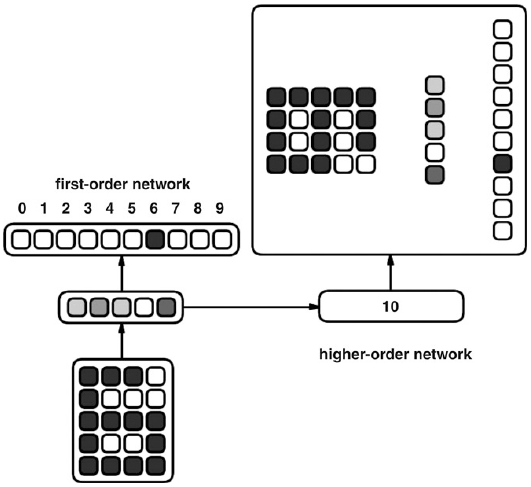
\includegraphics[width=220px]{data/expA1/schema.png}
      \end{center}
      
    \paragraph{Paramètres}
      \begin{center}
	\begin{tabular}{lr}
	  \begin{minipage}{230px}
	    \begin{itemize}
	      \item momentum : 0.9 sur les 2 réseaux
	      \item taux d'apprentissage : 0.1 sur les 2 réseaux
	      \item 10 chiffres différents présentés
	      \item apprentissage 10 (formes) x 4000 (époques)
	      \item utilisation de biais
	    \end{itemize}
	  \end{minipage}
	  &
	  \begin{minipage}{230px}
	    \begin{itemize}
	      \item poids initialisés sur [-0.25 ; 0.25]
	      \item taux d'apprentissage constant
	      \item entrées valent 0 ou 1
	      \item sigmoïde à température 1
	    \end{itemize}
	  \end{minipage}
	\end{tabular}
      \end{center}

  
  \newpage
  \subsection{Résultats}
    \paragraph{Principaux}
      Analyse des performances
      \begin{center}
	\begin{tabular}{lr}
	  \hspace*{-1cm}
	  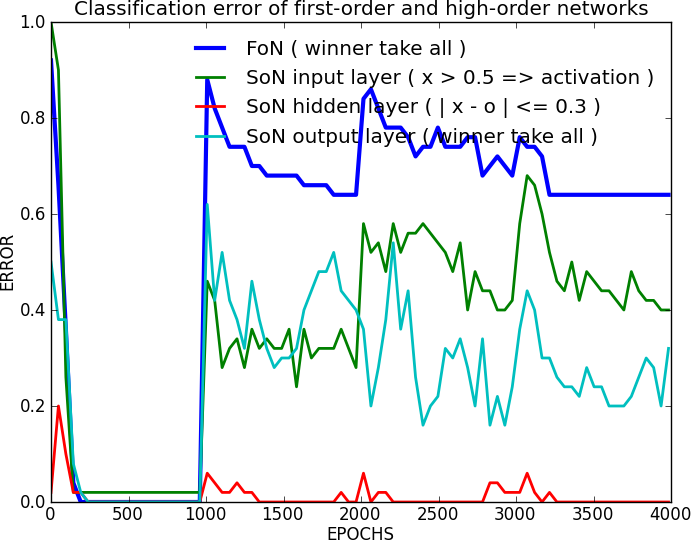
\includegraphics[width=250px]{data/expB1/err.png}
	  &
	  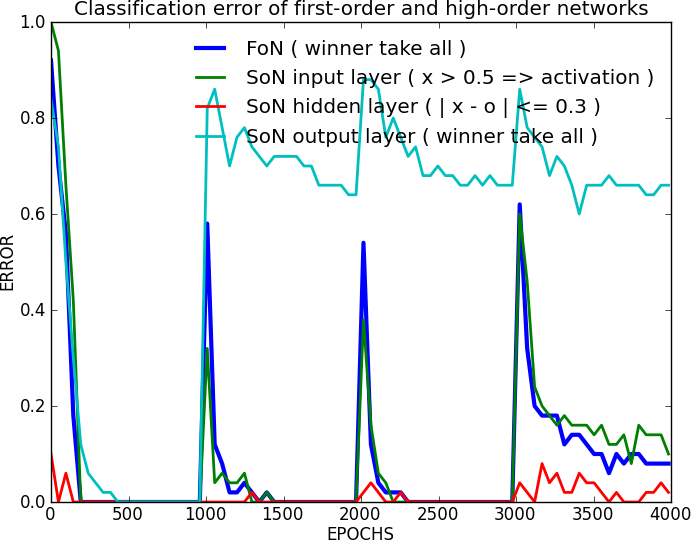
\includegraphics[width=250px]{data/expB1/err_block.png} \\
	  normal
	  &
	  poids figés
	\end{tabular}
      \end{center}
      \subparagraph{Notes}
	\begin{itemize}
	  \item l'erreur de classification représente le taux de mauvaises réponses pour les 10 formes présentées sur une époque
	  \item pour SoN input layer et hidden layer, un winner-take-all n'est pas possible (ce n'est pas de la classification, 
	  mais une duplication), il y a donc un seuil d'erreur qui ne doit pas être dépassé par un seul neurone
	\end{itemize}
      \subparagraph{Conclusion}
	\begin{itemize}
	  \item lorsque l'on fige les poids, le premier réseau arrive à se réadapter aux nouvelles tâches, mais s'ils ne sont
	  pas figés, il n'y arrive pas
	  \item la reproduction de la couche cachée par le second réseau ne pose pas de problème
	  \item lorsque l'on ne fige pas les poids, le second réseau est lui aussi instable
	  \item lorsque les poids sont figés, la couche de sortie a du mal à être totalement réapprise par le second réseau
	  
	\end{itemize}
    \paragraph{Secondaires}
      Analyse des performances RMS
      \begin{center}
	\begin{tabular}{lr}
	  \hspace*{-1cm}
	  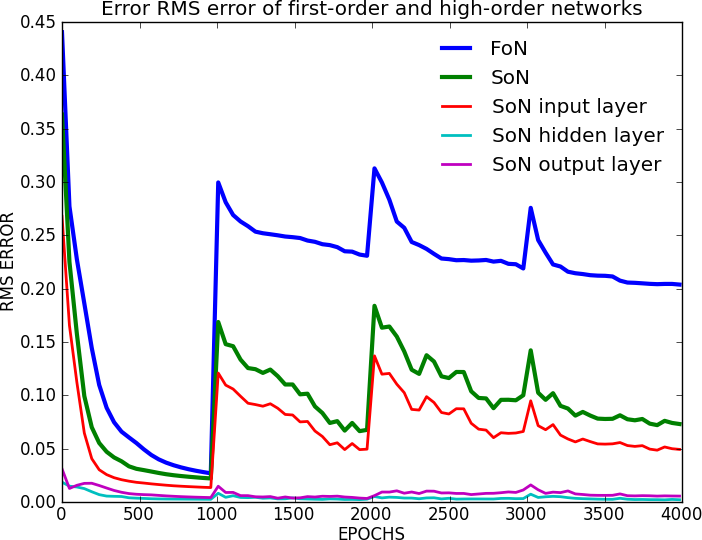
\includegraphics[width=250px]{data/expB1/rms.png}
	  &
	  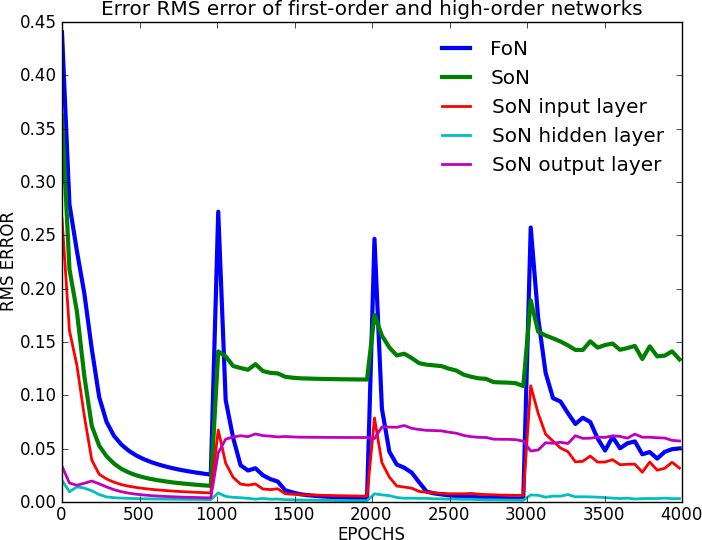
\includegraphics[width=250px]{data/expB1/rms_block.png} \\
	  normal 
	  &
	  poids figés
	\end{tabular}
      \end{center} 
      \subparagraph{Notes}
	\begin{itemize}
	  \item formule utilisée pour RMS (cf. Formules~\nameref{rms})
	  \item les courbes SoN layer représentent les erreurs (du second réseaux) sur les couches à reproduire 
	  \item la courbe RMS verte (SoN) est la somme des 3 courbes SoN layer
	\end{itemize}
      \subparagraph{Conclusion}
	Ces courbes sont a peu près équivalentes à celles de classifications.

  \subsection{Conclusion}
  Le blocage des poids dans la couche cachée prouve la présence de représentations stables permettant le 
  transfert de tâche.
  
  Ces représentations contiennent ce qui caractérise la forme sans encore lui mettre un sens dessus.
  Il sait à quoi ressemble un 1 (dans la couche cachée) et lui met un donne le sens 1 (dans la couche de sortie).
  Il est donc facile de lui dire que finalement, cette représentation correspond à un 2, sans qu'il ait à réapprendre
  la forme entièrement.
  
  

  \newpage 
  \subsection{Formules}
    \paragraph{RMS} \label{rms}
  Pour une époque $e$ :
  \begin{center}
    \begin{large}
    $ rms_{e} = \sqrt{ \frac{1}{n} \sum \limits_{i=1}^{n} 
    ( o_{i,e} - d_{i} )^2 } $
    \end{large}
  $ with \left\lbrace \begin{array}{lll} n : number\ of\ neurons\ on\ the\ output\ 
  layer\\o_{i,e} : value\ obtained\ for\ the\ i^{th}\ neuron\ at\ the\ e^{th}\ epoch\\d_{i} : 
  value\ desired \ for\ the\ i^{th}\ neuron\end{array} \right.$
  \end{center}
    \paragraph{Descente de gradient} \cite{Touzet_1992} \\
  Construction de l'erreur : 
    \begin{center}
      $y_{i} = f'(a_i) \times ( d_i - x_i ) \ si\ i\ neurone\ de\ sortie $ \\
      $y_{i} = f'(a_i) \times \sum \limits_{k} ( w_{ki} \times y_k )\ si\ i\ neurone\ cache $
    \end{center}
  Mise à jour des poids :
    \begin{center}
      $w_{ij}(t+1) = w_{ij}(t) + learning\_rate \times y_{i} \times x_j + momentum \times 
      (w_{ij}(t) - w_{ij}(t-1) )$
    \end{center}
  Variables : 
    \begin{center}
      $\left\lbrace \begin{array}{lll} 
	f : fonction\ sigmoide \\
	x_i : valeur\ du\ neurone\ i\\
	d_i : valeur\ desire pour\ le\ neurone\ i\\
	a_i : somme\ pondere\ des\ poids\ du\ neurone\ i
      \end{array} \right.$
    \end{center}

\bibliographystyle{../pre-rapport/apalike}
\bibliography{../pre-rapport/biblio}

  \section{Expérience B2} 
  \subsection{Objectif}
    Reproduction et approfondissement des résultats de la première expérience 1 dans l'article 
    \cite{Cleeremans_2007}. 

  
  
    Comprendre de quelles manières peuvent émerger des représentations et méta-représentations dans 
    un réseau de neurone connexionniste, en particulier sur des perceptrons multicouches.
  
  
  \subsection{Architecture}
    \paragraph{Description}
      Un premier réseau de perceptron multicouche apprend à discrétiser des chiffres représentés
      par 256 (16x16) neurones d'entrées. Il est composé d'une couche cachée de 64 neurones.
      
      Un second réseau de perceptron multicouche apprend à dupliquer toutes les couches du premier
      réseau en n'ayant que sa couche cachée en entrée.
      
      L'apprentissage du second réseau, n'affecte pas les poids entre la couche d'entrée et la 
      couche cachée du premier réseau.

    \paragraph{Schéma}
      \begin{center}
	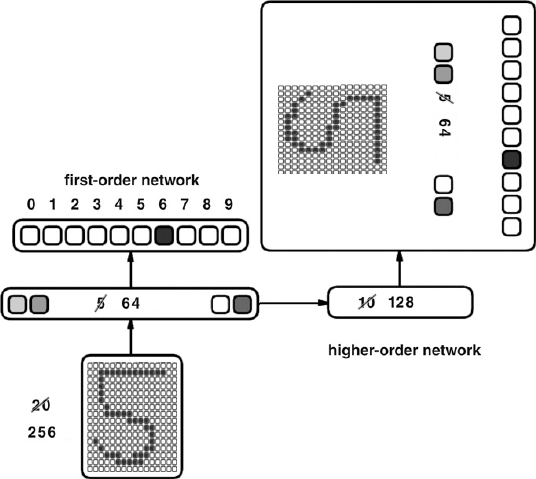
\includegraphics[width=220px]{data/expA3/schema.png}
      \end{center}
      
    \paragraph{Paramètres}
      \begin{center}
	\begin{tabular}{lr}
	  \begin{minipage}{230px}
	    \begin{itemize}
	      \item momentum : 0.9 sur les 2 réseaux
	      \item taux d'apprentissage : 0.1 sur les 2 réseaux
	      \item \textbf{1600 formes} de chiffres différents présentées (shuffle) \cite{Handwritten_256}
	      \item apprentissage 10 (formes) x 1000 (époques)
	    \end{itemize}
	  \end{minipage}
	  &
	  \begin{minipage}{230px}
	    \begin{itemize}
	      \item poids initialisés sur [-0.25 ; 0.25]
	      \item taux d'apprentissage constant
	      \item entrées valent 0 ou 1
	      \item sigmoïde à température 1
	      \item utilisation de biais
	    \end{itemize}
	  \end{minipage}
	\end{tabular}
      \end{center}

  
  \newpage
  \subsection{Résultats}
    \paragraph{Principaux}
      Analyse des performances
      \begin{center}
	\begin{tabular}{lr}
	  \hspace*{-1cm}
	  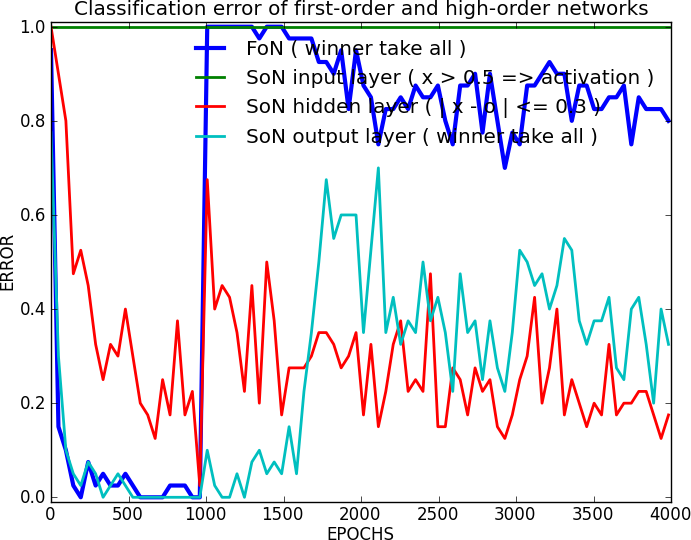
\includegraphics[width=250px]{data/expB2/err.png}
	  &
	  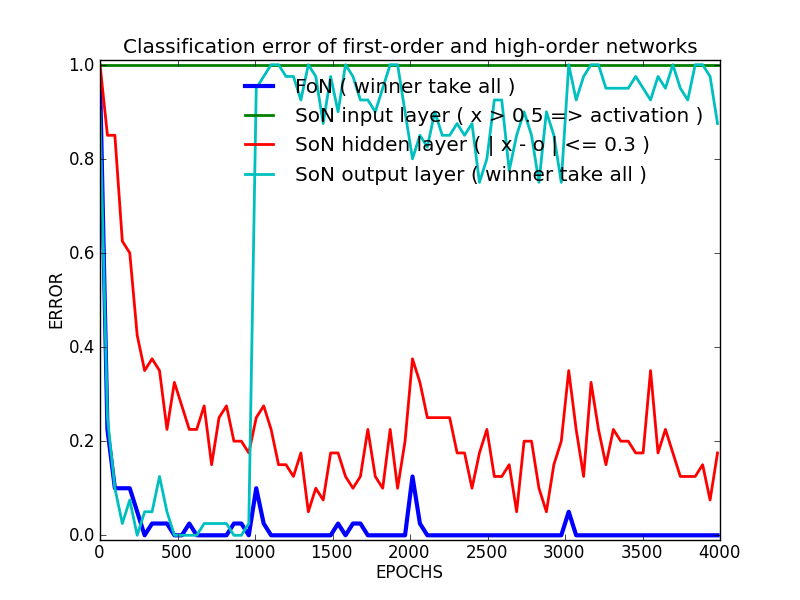
\includegraphics[width=250px]{data/expB2/err_block.png} 
	\end{tabular}
      \end{center}
      \subparagraph{Notes}
	\begin{itemize}
	  \item les courbes SoN layer représentent les erreurs (du second réseaux) des couches du premier à reproduire 
	  \item la courbe RMS verte (SoN) est la somme des 3 courbes SoN layer
	\end{itemize}
      \subparagraph{Conclusion}
	\begin{itemize}
	  \item la couche cachée et la couche de sortie ne posent aucun problèmes d'apprentissage
	  \item les performances du second réseau dépendent principalement de sa capacité à reproduire les entrées
	  \item le second réseau apprend plus rapidement que le premier
	\end{itemize}
    \paragraph{Secondaires}
      RMS
      \begin{center}
	\begin{tabular}{lr}
	  \hspace*{-1cm}
	  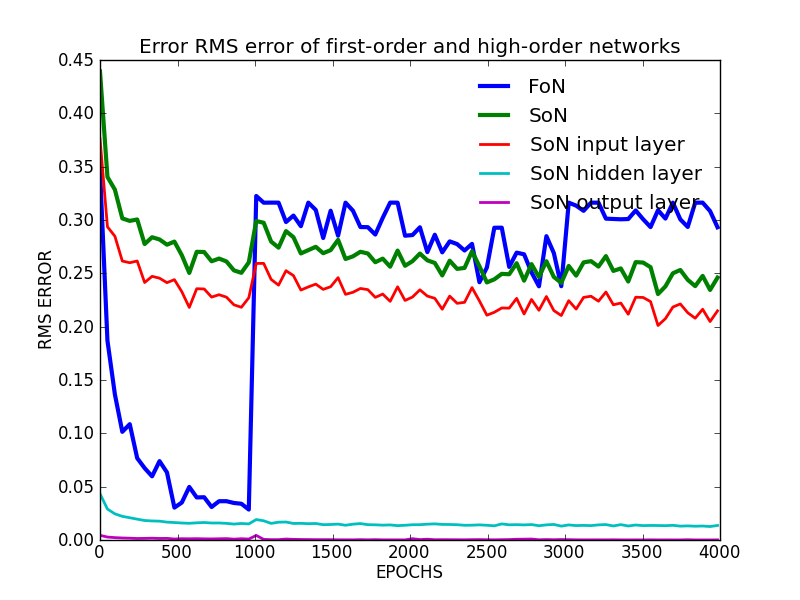
\includegraphics[width=250px]{data/expB2/rms.png}
	  &
	  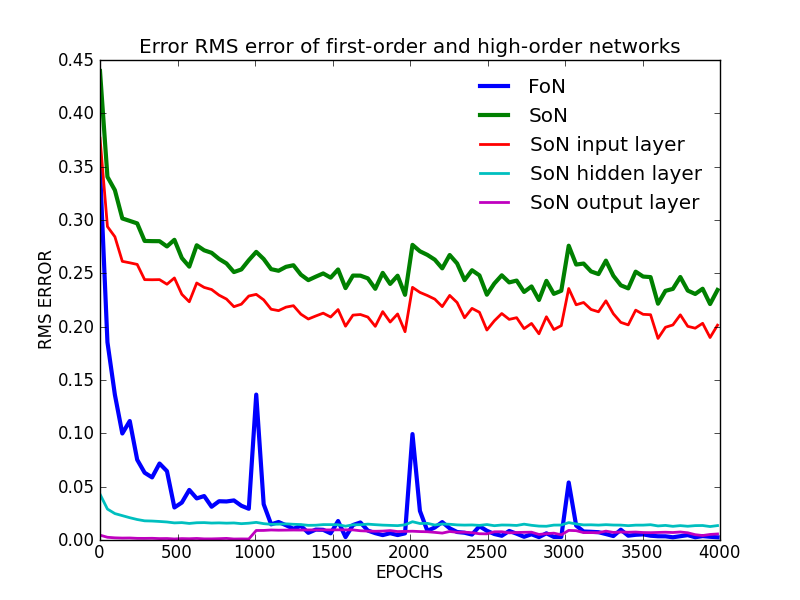
\includegraphics[width=250px]{data/expB2/rms_block.png} 
	\end{tabular}
      \end{center} 
      \subparagraph{Notes}
	\begin{itemize}
	  \item une couleur équivaut à un chiffre présenté
	  \item une valeur discretisée correspond à un certain encodage de la couche cachée (cf Algorithmes)
	\end{itemize}
      \subparagraph{Conclusion}
	Les neurones se stabilisent très rapidement (autour de la 50\up{ième} époque en moyenne), 
	le tout permettant au second réseau d'avoir des entrées très peu variables, favorisant
	son apprentissage.

  \subsection{Conclusion}
  
  

  \newpage 
  \subsection{Formules}
    \paragraph{RMS} \label{rms}
  Pour une époque $e$ :
  \begin{center}
    \begin{large}
    $ rms_{e} = \sqrt{ \frac{1}{n} \sum \limits_{i=1}^{n} 
    ( o_{i,e} - d_{i} )^2 } $
    \end{large}
  $ with \left\lbrace \begin{array}{lll} n : number\ of\ neurons\ on\ the\ output\ 
  layer\\o_{i,e} : value\ obtained\ for\ the\ i^{th}\ neuron\ at\ the\ e^{th}\ epoch\\d_{i} : 
  value\ desired \ for\ the\ i^{th}\ neuron\end{array} \right.$
  \end{center}
    \paragraph{Discrétisation} \label{discretize}
      Pour la couche cachée $hiddenNeuron$ de $n$ neurones, un neurone
      pouvant être encodé par $number\_cutting$ valeurs différentes :
      \begin{center}
	$\sum \limits_{i=0}^{n} number\_cutting^{i} \times cutting(hiddenNeuron[i]) $
      \end{center}
      \subparagraph{Exemple}
	$400 \gets [0 ; 0,25 ]\ [0 ; 0,25 ]\  [0,25 ; 0,5 ]\  [0,5 ; 0,75 ]\  [0,25 ; 0,5 ]$ \\
	\hspace*{2.70cm}
	$400 \gets 0\times4^0 +   0\times4^1  +   1\times4^2   +  2\times4^3   +   1 \times4^4$
    \paragraph{Descente de gradient} \cite{Touzet_1992} \\
  Construction de l'erreur : 
    \begin{center}
      $y_{i} = f'(a_i) \times ( d_i - x_i ) \ si\ i\ neurone\ de\ sortie $ \\
      $y_{i} = f'(a_i) \times \sum \limits_{k} ( w_{ki} \times y_k )\ si\ i\ neurone\ cache $
    \end{center}
  Mise à jour des poids :
    \begin{center}
      $w_{ij}(t+1) = w_{ij}(t) + learning\_rate \times y_{i} \times x_j + momentum \times 
      (w_{ij}(t) - w_{ij}(t-1) )$
    \end{center}
  Variables : 
    \begin{center}
      $\left\lbrace \begin{array}{lll} 
	f : fonction\ sigmoide \\
	x_i : valeur\ du\ neurone\ i\\
	d_i : valeur\ desire pour\ le\ neurone\ i\\
	a_i : somme\ pondere\ des\ poids\ du\ neurone\ i
      \end{array} \right.$
    \end{center}

\bibliographystyle{../pre-rapport/apalike}
\bibliography{../pre-rapport/biblio}

  \section{Expérience B3} 
  \subsection{Objectif}
    Reproduction et approfondissement des résultats de la première expérience 1 dans l'article 
    \cite{Cleeremans_2007}. 

  
  
    Comprendre de quelles manières peuvent émerger des représentations et méta-représentations dans 
    un réseau de neurone connexionniste, en particulier sur des perceptrons multicouches.
  
  
  \subsection{Architecture}
    \paragraph{Description}
      Un premier réseau de perceptron multicouche apprend à discrétiser des chiffres représentés
      par 20 neurones d'entrées. Il est composé d'une couche cachée de 5 neurones.
      
      Un second réseau de perceptron multicouche apprend à dupliquer toutes les couches du premier
      réseau en n'ayant que sa couche cachée en entrée.
      
      L'apprentissage du second réseau, n'affecte pas les poids entre la couche d'entrée et la 
      couche cachée du premier réseau.

    \paragraph{Schéma}
      \begin{center}
	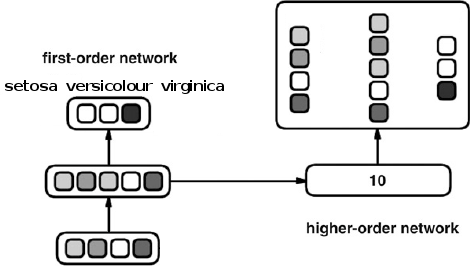
\includegraphics[width=220px]{data/expA4/schema.png}
      \end{center}
      
    \paragraph{Paramètres}
      \begin{center}
	\begin{tabular}{lr}
	  \begin{minipage}{230px}
	    \begin{itemize}
	      \item momentum : 0.9 sur les 2 réseaux
	      \item taux d'apprentissage : 0.1 sur les 2 réseaux
	      \item 10 chiffres différents présentés
	      \item apprentissage 10 (formes) x 1000 (époques)
	      \item utilisation de biais
	    \end{itemize}
	  \end{minipage}
	  &
	  \begin{minipage}{230px}
	    \begin{itemize}
	      \item poids initialisés sur [-0.25 ; 0.25]
	      \item taux d'apprentissage constant
	      \item entrées valent 0 ou 1
	      \item sigmoïde à température 1
	    \end{itemize}
	  \end{minipage}
	\end{tabular}
      \end{center}

  
  \newpage
  \subsection{Résultats}
    \paragraph{Principaux}
      Analyse des performances
      \begin{center}
	\begin{tabular}{lr}
	  \hspace*{-1cm}
	  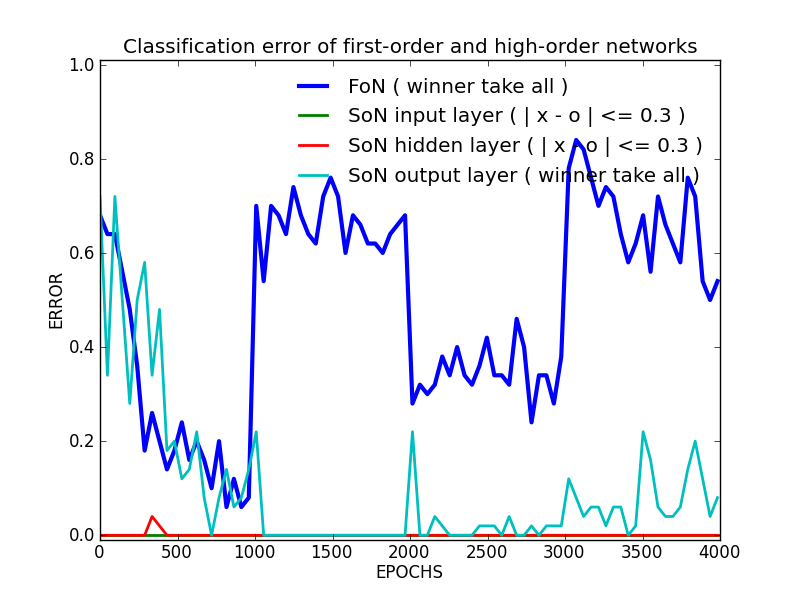
\includegraphics[width=250px]{data/expB3/err.png}
	  &
	  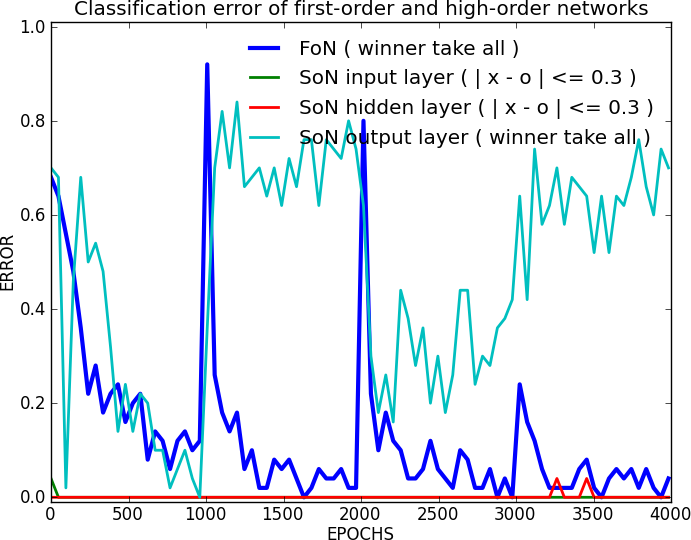
\includegraphics[width=250px]{data/expB3/err_block.png} 
	\end{tabular}
      \end{center}
      \subparagraph{Notes}
	\begin{itemize}
	  \item les courbes SoN layer représentent les erreurs (du second réseaux) des couches du premier à reproduire 
	  \item la courbe RMS verte (SoN) est la somme des 3 courbes SoN layer
	\end{itemize}
      \subparagraph{Conclusion}
	\begin{itemize}
	  \item la couche cachée et la couche de sortie ne posent aucun problèmes d'apprentissage
	  \item les performances du second réseau dépendent principalement de sa capacité à reproduire les entrées
	  \item le second réseau apprend plus rapidement que le premier
	\end{itemize}
    \paragraph{Secondaires}
      RMS
      \begin{center}
	\begin{tabular}{lr}
	  \hspace*{-1cm}
	  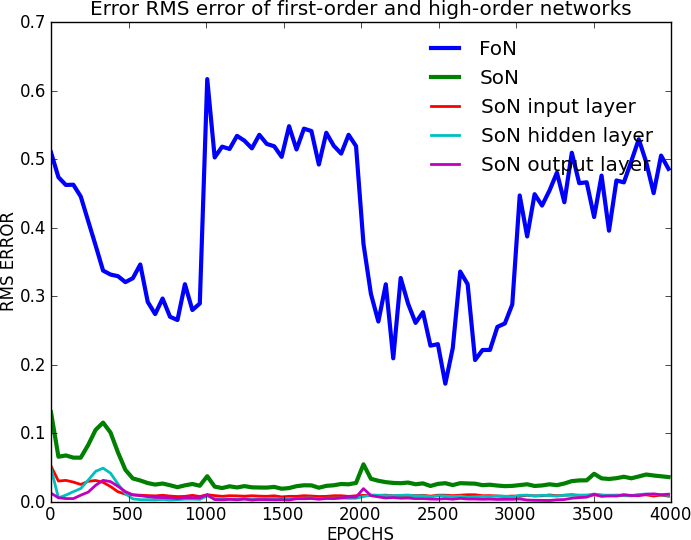
\includegraphics[width=250px]{data/expB3/rms.png}
	  &
	  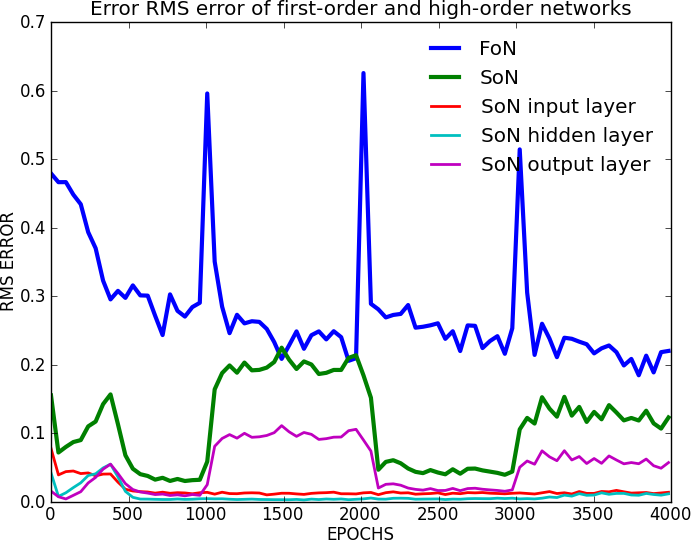
\includegraphics[width=250px]{data/expB3/rms_block.png} 
	\end{tabular}
      \end{center} 
      \subparagraph{Notes}
	\begin{itemize}
	  \item une couleur équivaut à un chiffre présenté
	  \item une valeur discretisée correspond à un certain encodage de la couche cachée (cf Algorithmes)
	\end{itemize}
      \subparagraph{Conclusion}
	Les neurones se stabilisent très rapidement (autour de la 50\up{ième} époque en moyenne), 
	le tout permettant au second réseau d'avoir des entrées très peu variables, favorisant
	son apprentissage.
    \paragraph{Secondaires}
      Représentations au travers des poids du premier réseau
      \begin{center}
	Couche cachée \\
	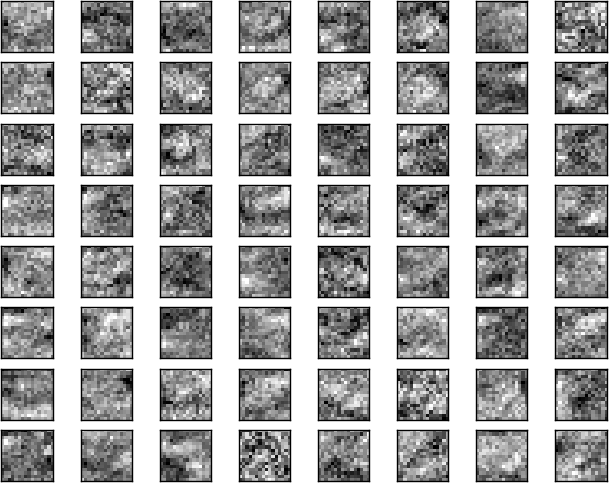
\includegraphics[width=250px]{data/expA3/representation_hidden.png}
      \end{center}
      \begin{center}
	Couche de sortie \\
	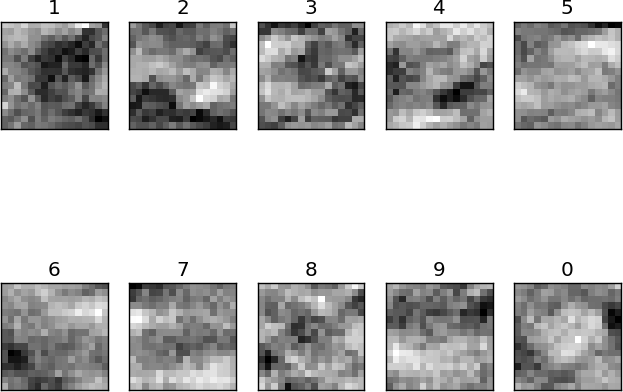
\includegraphics[width=250px]{data/expA3/representation.png}
      \end{center} 
      \subparagraph{Notes}
	\begin{itemize}
	  \item plus une case est noire, plus sa présence est importante pour le chiffre en question
	  \item plus une case est blanche, plus son absence est importante
	\end{itemize}
      \subparagraph{Conclusion}
	Il est assez difficile d'y distinquer les chiffres, mais cela semble suffisant pour le réseau
	qui a un taux de reconnaissance de 100\%.

      \subparagraph{Conclusion}
	Le peu d'entrées permet l'apprentissage par-coeur de chaque forme.
	


  \subsection{Conclusion}
  
  

  \newpage 
  \subsection{Formules}
    \paragraph{RMS} \label{rms}
  Pour une époque $e$ :
  \begin{center}
    \begin{large}
    $ rms_{e} = \sqrt{ \frac{1}{n} \sum \limits_{i=1}^{n} 
    ( o_{i,e} - d_{i} )^2 } $
    \end{large}
  $ with \left\lbrace \begin{array}{lll} n : number\ of\ neurons\ on\ the\ output\ 
  layer\\o_{i,e} : value\ obtained\ for\ the\ i^{th}\ neuron\ at\ the\ e^{th}\ epoch\\d_{i} : 
  value\ desired \ for\ the\ i^{th}\ neuron\end{array} \right.$
  \end{center}
    \paragraph{Discrétisation} \label{discretize}
      Pour la couche cachée $hiddenNeuron$ de $n$ neurones, un neurone
      pouvant être encodé par $number\_cutting$ valeurs différentes :
      \begin{center}
	$\sum \limits_{i=0}^{n} number\_cutting^{i} \times cutting(hiddenNeuron[i]) $
      \end{center}
      \subparagraph{Exemple}
	$400 \gets [0 ; 0,25 ]\ [0 ; 0,25 ]\  [0,25 ; 0,5 ]\  [0,5 ; 0,75 ]\  [0,25 ; 0,5 ]$ \\
	\hspace*{2.70cm}
	$400 \gets 0\times4^0 +   0\times4^1  +   1\times4^2   +  2\times4^3   +   1 \times4^4$
    \paragraph{Descente de gradient} \cite{Touzet_1992} \\
  Construction de l'erreur : 
    \begin{center}
      $y_{i} = f'(a_i) \times ( d_i - x_i ) \ si\ i\ neurone\ de\ sortie $ \\
      $y_{i} = f'(a_i) \times \sum \limits_{k} ( w_{ki} \times y_k )\ si\ i\ neurone\ cache $
    \end{center}
  Mise à jour des poids :
    \begin{center}
      $w_{ij}(t+1) = w_{ij}(t) + learning\_rate \times y_{i} \times x_j + momentum \times 
      (w_{ij}(t) - w_{ij}(t-1) )$
    \end{center}
  Variables : 
    \begin{center}
      $\left\lbrace \begin{array}{lll} 
	f : fonction\ sigmoide \\
	x_i : valeur\ du\ neurone\ i\\
	d_i : valeur\ desire pour\ le\ neurone\ i\\
	a_i : somme\ pondere\ des\ poids\ du\ neurone\ i
      \end{array} \right.$
    \end{center}

\bibliographystyle{../pre-rapport/apalike}
\bibliography{../pre-rapport/biblio}

  \section{Expérience C1} 
  \subsection{Résumé}
    Reproduction et approfondissement des résultats de la première expérience 1 dans l'article 
    \cite{Cleeremans_2007}. 

  
  \subsection{But}
    Comprendre de quelles manières peuvent émerger des représentations et méta-représentations dans 
    un réseau de neurone connexionniste, en particulier sur des perceptrons multicouches.
  
  
  \subsection{Architecture}
    \paragraph{Description}
      Un premier réseau de perceptron multicouche apprend à discrétiser des chiffres représentés
      par 20 neurones d'entrées. Il est composé d'une couche cachée de 5 neurones.
      
      Un second réseau de perceptron multicouche apprend à dupliquer toutes les couches du premier
      réseau en n'ayant que sa couche cachée en entrée.
      
      L'apprentissage du second réseau, n'affecte pas les poids entre la couche d'entrée et la 
      couche cachée du premier réseau.

    \paragraph{Schéma}
      \begin{center}
	\includegraphics[width=220px]{data/expC1/schema.png}
      \end{center}
      
    \paragraph{Paramètres}
      \begin{center}
	\begin{tabular}{lr}
	  \begin{minipage}{220px}
	    \begin{itemize}
	      \item momentum : 0.9 sur les 2 réseau
	      \item taux d'apprentissage : 0.1 sur les 2 réseau
	      \item 10 chiffres différents présentés
	      \item apprentissage 10 (formes) x 1000 (époques)
	      \item utilisation de biais
	    \end{itemize}
	  \end{minipage}
	  &
	  \begin{minipage}{205px}
	    \begin{itemize}
	      \item poids initialisés sur [-0.25 ; 0.25]
	      \item taux d'apprentissage constant
	      \item entrées valent 0 ou 1
	      \item sigmoïde à température 1
	    \end{itemize}
	  \end{minipage}
	\end{tabular}
      \end{center}

  
  \newpage
  \subsection{Résultats}
    \paragraph{Principaux}
      Analyse des performances
      \begin{center}
	\begin{tabular}{lr}
	  \hspace*{-1cm}
	  \includegraphics[width=250px]{data/expC1/perf_20.png}
	  &
	  \includegraphics[width=250px]{data/expC1/perf_100.png} 
	\end{tabular}
      \end{center}
      \subparagraph{Notes}
	\begin{itemize}
	  \item les courbes SoN layer représentent les erreurs (du second réseaux) des couches du premier à reproduire 
	  \item la courbe RMS verte (SoN) est la somme des 3 courbes SoN layer
	\end{itemize}
      \subparagraph{Conclusion}
	\begin{itemize}
	  \item la couche cachée et la couche de sortie ne posent aucun problèmes d'apprentissage
	  \item les performances du second réseau dépendent principalement de sa capacité à reproduire les entrées
	  \item le second réseau apprend plus rapidement que le premier
	\end{itemize}
    \paragraph{Secondaires}
      RMS
      \begin{center}
	\begin{tabular}{lr}
	  \hspace*{-1cm}
	  \includegraphics[width=250px]{data/expC1/rms_20.png}
	  &
	  \includegraphics[width=250px]{data/expC1/rms_100.png} 
	\end{tabular}
      \end{center} 
      \subparagraph{Notes}
	\begin{itemize}
	  \item une couleur équivaut à un chiffre présenté
	  \item une valeur discretisée correspond à un certain encodage de la couche cachée (cf Algorithmes)
	\end{itemize}
      \subparagraph{Conclusion}
	Les neurones se stabilisent très rapidement (autour de la 50\up{ième} époque en moyenne), 
	le tout permettant au second réseau d'avoir des entrées très peu variables, favorisant
	son apprentissage.


  \subsection{Conclusion}
  
  

  \newpage 
  \subsection{Formules}
    \paragraph{RMS} \label{rms}
  Pour une époque $e$ :
  \begin{center}
    \begin{large}
    $ rms_{e} = \sqrt{ \frac{1}{n} \sum \limits_{i=1}^{n} 
    ( o_{i,e} - d_{i} )^2 } $
    \end{large}
  $ with \left\lbrace \begin{array}{lll} n : number\ of\ neurons\ on\ the\ output\ 
  layer\\o_{i,e} : value\ obtained\ for\ the\ i^{th}\ neuron\ at\ the\ e^{th}\ epoch\\d_{i} : 
  value\ desired \ for\ the\ i^{th}\ neuron\end{array} \right.$
  \end{center}
    \paragraph{Discrétisation} \label{discretize}
      Pour la couche cachée $hiddenNeuron$ de $n$ neurones, un neurone
      pouvant être encodé par $number\_cutting$ valeurs différentes :
      \begin{center}
	$\sum \limits_{i=0}^{n} number\_cutting^{i} \times cutting(hiddenNeuron[i]) $
      \end{center}
      \subparagraph{Exemple}
	$400 \gets [0 ; 0,25 ]\ [0 ; 0,25 ]\  [0,25 ; 0,5 ]\  [0,5 ; 0,75 ]\  [0,25 ; 0,5 ]$ \\
	\hspace*{2.70cm}
	$400 \gets 0\times4^0 +   0\times4^1  +   1\times4^2   +  2\times4^3   +   1 \times4^4$
    \paragraph{Descente de gradient} \cite{Touzet_1992} \\
  Construction de l'erreur : 
    \begin{center}
      $y_{i} = f'(a_i) \times ( d_i - x_i ) \ si\ i\ neurone\ de\ sortie $ \\
      $y_{i} = f'(a_i) \times \sum \limits_{k} ( w_{ki} \times y_k )\ si\ i\ neurone\ cache $
    \end{center}
  Mise à jour des poids :
    \begin{center}
      $w_{ij}(t+1) = w_{ij}(t) + learning\_rate \times y_{i} \times x_j + momentum \times 
      (w_{ij}(t) - w_{ij}(t-1) )$
    \end{center}
  Variables : 
    \begin{center}
      $\left\lbrace \begin{array}{lll} 
	f : fonction\ sigmoide \\
	x_i : valeur\ du\ neurone\ i\\
	d_i : valeur\ desire pour\ le\ neurone\ i\\
	a_i : somme\ pondere\ des\ poids\ du\ neurone\ i
      \end{array} \right.$
    \end{center}
    
\bibliographystyle{../pre-rapport/apalike}
\bibliography{../pre-rapport/biblio}

  \section{Expérience C2} \label{expC2}
  \subsection{Objectif}
    Comprendre de quelles manières un réseau de neurone connexionniste peut parier sur ses propres résultats
    à partir de ses représentations personnelles.

    
    Réalisation de la seconde expérience de l'article \cite{Cleeremans_2007} sur des données réelles.
  
  
  \subsection{Architecture}
    \paragraph{Description}
      Un premier réseau de perceptron multicouche apprend à discrétiser des chiffres représentés
      par 256 (16x16) neurones d'entrées. Il est composé d'une couche cachée de 20 ou 100 neurones.
      
      Un second réseau de perceptron multicouche apprend à parier sur la qualité de la réponse
      du premier réseau à partir de sa couche cachée.
      
      L'apprentissage du second réseau, n'affecte pas les poids entre la couche d'entrée et la 
      couche cachée du premier réseau.

    \paragraph{Schéma}
      \begin{center}
	\includegraphics[width=240px]{data/expC2/schema.png}
      \end{center}
      
    \paragraph{Paramètres}
      \begin{center}
	\begin{tabular}{lr}
	  \begin{minipage}{230px}
	    \begin{itemize}
	      \item momentum : 0.5 sur le premier réseau
	      \item momentum : 0. sur le second réseau
	      \item taux d'apprentissage : 0.15 sur les 2 réseaux
	      \item \textbf{1600 formes} de chiffres différents présentées (shuffle) \cite{Handwritten_256}
	      \item apprentissage 50 (formes) x 300 (époques)
	      \item utilisation de biais
	      
	    \end{itemize}
	  \end{minipage}
	  &
	  \begin{minipage}{230px}
	    \begin{itemize}
	      \item poids initialisés sur [-1 ; 1] pour le premier réseau
	      \item poids initialisés sur [-0.25 ; 0.25] pour le second réseau
	      \item taux d'apprentissage constant
	      \item entrées valent 0 ou 1
	      \item sigmoïde à température 1
	    \end{itemize}
	  \end{minipage}
	\end{tabular}
      \end{center}


  
  \newpage
  \subsection{Résultats}
    \paragraph{Principaux}
      Analyse des performances
      \begin{center}
	\begin{tabular}{lr}
	  \hspace*{-1cm}
	  \includegraphics[width=250px]{data/expC2/perf_20.png}
	  &
	  \includegraphics[width=250px]{data/expC2/perf_100.png} \\
	  
	  20 neurones en couche cachée
	  &
	  \hspace*{-1cm}
	  100 neurones en couche cachée
	\end{tabular}
      \end{center}
      \subparagraph{Notes}
	\begin{itemize}
	  \item la performance de classification représente le taux de bonnes réponses (winner-take-all) pour les 50 formes présentées sur une époque
	  \item la courbe rouge représentent le taux de paris hauts du second réseau
	\end{itemize}
      \subparagraph{Conclusion}
	\begin{itemize}
	  \item dans les 2 cas, le premier réseau réussit à apprendre sa tâche de classification
	  \item lorsque le nombre de neurones dans la couche cachée est faible, l'apprentissage de la tâche est optimal, il ne peut plus être amélioré
	  
	  Ainsi le second réseau se contente de parier haut.
	  \item lorsque le nombre de neurones dans la couche cachée est élevé, l'apprentissage peut être amélioré, le second réseau 
	  le remarque et peut accorder son taux de paris hauts avec le taux de succès du premier réseau.
	  
	  Remarquons tout de même qu'avec l'amélioration du second réseau, on ne peut pas dépasser un réseau optimal, seulement l'égaler
	\end{itemize}
    \paragraph{Secondaires}
      RMS
      \begin{center}
	\begin{tabular}{lr}
	  \hspace*{-1cm}
	  \includegraphics[width=250px]{data/expC2/rms_20.png}
	  &
	  \includegraphics[width=250px]{data/expC2/rms_100.png} \\
	  
	  20 neurones en couche cachée
	  &
	  \hspace*{-1cm}
	  100 neurones en couche cachée
	\end{tabular}
      \end{center} 
      \subparagraph{Notes}
	\begin{itemize}
	  \item formule utilisée pour RMS (cf. Formules~\nameref{rms})
	\end{itemize}
      \subparagraph{Conclusion}
	On remarque que le second réseau apprend et désapprend. De plus, il reste toujours sous la barre
	des 0.5.


  \subsection{Conclusion}
      Comme il l'est dit dans \cite{Cleeremans_2007}, cette architecture tente de résoudre les problèmes des réseaux connexionnistes
    classiques à avoir un semblant de conscience.
    
    À savoir :
    \begin{itemize}
    \item qu'ils ne savent pas qu'ils peuvent se trouver dans différents états, et qu'ils ne traitent pas leurs propres états : 
    d'où la présence de ce second réseau qui tente de traiter ses états et d'apprendre qu'il en a plusieurs
    \item des représentations rentant bloquées dans la chaîne de causalité de la tâche à apprendre : d'où
    le fait que ce second réseau n'affecte pas l'apprentissage du premier (ie. pour ne pas retomber dans la chaîne de causalité)
    \item qu'ils n'ont pas les connaissances conscientes des raisons de leurs décisions : on essaye de les y sensibiliser avec les paris
    \\[0.2cm]
    \end{itemize}
  
    Le passage sur des données réelles ne modifient pas le comportement du réseau.
    
    
    Par ailleurs, cette architecture ouvre des possibilités d'amélioration de l'apprentissage.
    Elle permet au réseau de détecter lui même un nombre de neurones trop important dans la couche cachée.
    On pourrait, par exemple, imaginer un réseau autorégulant son nombre de neurone.
    
    Toutes les expériences F et G découlent de cette architecture.
  

  \newpage 
  \subsection{Formules}
    \paragraph{RMS} \label{rms}
  Pour une époque $e$ :
  \begin{center}
    \begin{large}
    $ rms_{e} = \sqrt{ \frac{1}{n} \sum \limits_{i=1}^{n} 
    ( o_{i,e} - d_{i} )^2 } $
    \end{large}
  $ with \left\lbrace \begin{array}{lll} n : number\ of\ neurons\ on\ the\ output\ 
  layer\\o_{i,e} : value\ obtained\ for\ the\ i^{th}\ neuron\ at\ the\ e^{th}\ epoch\\d_{i} : 
  value\ desired \ for\ the\ i^{th}\ neuron\end{array} \right.$
  \end{center}
    \paragraph{Descente de gradient} \cite{Touzet_1992} \\
  Construction de l'erreur : 
    \begin{center}
      $y_{i} = f'(a_i) \times ( d_i - x_i ) \ si\ i\ neurone\ de\ sortie $ \\
      $y_{i} = f'(a_i) \times \sum \limits_{k} ( w_{ki} \times y_k )\ si\ i\ neurone\ cache $
    \end{center}
  Mise à jour des poids :
    \begin{center}
      $w_{ij}(t+1) = w_{ij}(t) + learning\_rate \times y_{i} \times x_j + momentum \times 
      (w_{ij}(t) - w_{ij}(t-1) )$
    \end{center}
  Variables : 
    \begin{center}
      $\left\lbrace \begin{array}{lll} 
	f : fonction\ sigmoide \\
	x_i : valeur\ du\ neurone\ i\\
	d_i : valeur\ desire pour\ le\ neurone\ i\\
	a_i : somme\ pondere\ des\ poids\ du\ neurone\ i
      \end{array} \right.$
    \end{center}
    
\bibliographystyle{../pre-rapport/apalike}
\bibliography{../pre-rapport/biblio}

  \section{Expérience C3} 
  \subsection{Objectif}
    Reproduction et approfondissement des résultats de la première expérience 1 dans l'article 
    \cite{Cleeremans_2007}. 

  
  
    Comprendre de quelles manières peuvent émerger des représentations et méta-représentations dans 
    un réseau de neurone connexionniste, en particulier sur des perceptrons multicouches.
  
  
  \subsection{Architecture}
    \paragraph{Description}
      Un premier réseau de perceptron multicouche apprend à discrétiser des chiffres représentés
      par 20 neurones d'entrées. Il est composé d'une couche cachée de 5 neurones.
      
      Un second réseau de perceptron multicouche apprend à dupliquer toutes les couches du premier
      réseau en n'ayant que sa couche cachée en entrée.
      
      L'apprentissage du second réseau, n'affecte pas les poids entre la couche d'entrée et la 
      couche cachée du premier réseau.

    \paragraph{Schéma}
      \begin{center}
	\includegraphics[width=220px]{data/expC3/schema.png}
      \end{center}
      
    \paragraph{Paramètres}
      \begin{center}
	\begin{tabular}{lr}
	  \begin{minipage}{220px}
	    \begin{itemize}
	      \item momentum : 0.9 sur les 2 réseau
	      \item taux d'apprentissage : 0.1 sur les 2 réseau
	      \item 10 chiffres différents présentés
	      \item apprentissage 10 (formes) x 1000 (époques)
	      \item utilisation de biais
	    \end{itemize}
	  \end{minipage}
	  &
	  \begin{minipage}{205px}
	    \begin{itemize}
	      \item poids initialisés sur [-0.25 ; 0.25]
	      \item taux d'apprentissage constant
	      \item entrées valent 0 ou 1
	      \item sigmoïde à température 1
	    \end{itemize}
	  \end{minipage}
	\end{tabular}
      \end{center}

  
  \newpage
  \subsection{Résultats}
    \paragraph{Principaux}
      Analyse des performances
      \begin{center}
	\begin{tabular}{lr}
	  \hspace*{-1cm}
	  \includegraphics[width=250px]{data/expC3/perf_5.png}
	  &
	  \includegraphics[width=250px]{data/expC3/perf_100.png} 
	\end{tabular}
      \end{center}
      \subparagraph{Notes}
	\begin{itemize}
	  \item les courbes SoN layer représentent les erreurs (du second réseaux) des couches du premier à reproduire 
	  \item la courbe RMS verte (SoN) est la somme des 3 courbes SoN layer
	\end{itemize}
      \subparagraph{Conclusion}
	\begin{itemize}
	  \item la couche cachée et la couche de sortie ne posent aucun problèmes d'apprentissage
	  \item les performances du second réseau dépendent principalement de sa capacité à reproduire les entrées
	  \item le second réseau apprend plus rapidement que le premier
	\end{itemize}
    \paragraph{Secondaires}
      RMS
      \begin{center}
	\begin{tabular}{lr}
	  \hspace*{-1cm}
	  \includegraphics[width=250px]{data/expC3/rms_5.png}
	  &
	  \includegraphics[width=250px]{data/expC3/rms_100.png} 
	\end{tabular}
      \end{center} 
      \subparagraph{Notes}
	\begin{itemize}
	  \item une couleur équivaut à un chiffre présenté
	  \item une valeur discretisée correspond à un certain encodage de la couche cachée (cf Algorithmes)
	\end{itemize}
      \subparagraph{Conclusion}
	Les neurones se stabilisent très rapidement (autour de la 50\up{ième} époque en moyenne), 
	le tout permettant au second réseau d'avoir des entrées très peu variables, favorisant
	son apprentissage.


  \subsection{Conclusion}
  
  

  \newpage 
  \subsection{Formules}
    \paragraph{RMS} \label{rms}
  Pour une époque $e$ :
  \begin{center}
    \begin{large}
    $ rms_{e} = \sqrt{ \frac{1}{n} \sum \limits_{i=1}^{n} 
    ( o_{i,e} - d_{i} )^2 } $
    \end{large}
  $ with \left\lbrace \begin{array}{lll} n : number\ of\ neurons\ on\ the\ output\ 
  layer\\o_{i,e} : value\ obtained\ for\ the\ i^{th}\ neuron\ at\ the\ e^{th}\ epoch\\d_{i} : 
  value\ desired \ for\ the\ i^{th}\ neuron\end{array} \right.$
  \end{center}
    
    \paragraph{Descente de gradient} \cite{Touzet_1992} \\
  Construction de l'erreur : 
    \begin{center}
      $y_{i} = f'(a_i) \times ( d_i - x_i ) \ si\ i\ neurone\ de\ sortie $ \\
      $y_{i} = f'(a_i) \times \sum \limits_{k} ( w_{ki} \times y_k )\ si\ i\ neurone\ cache $
    \end{center}
  Mise à jour des poids :
    \begin{center}
      $w_{ij}(t+1) = w_{ij}(t) + learning\_rate \times y_{i} \times x_j + momentum \times 
      (w_{ij}(t) - w_{ij}(t-1) )$
    \end{center}
  Variables : 
    \begin{center}
      $\left\lbrace \begin{array}{lll} 
	f : fonction\ sigmoide \\
	x_i : valeur\ du\ neurone\ i\\
	d_i : valeur\ desire pour\ le\ neurone\ i\\
	a_i : somme\ pondere\ des\ poids\ du\ neurone\ i
      \end{array} \right.$
    \end{center}
    
\bibliographystyle{../pre-rapport/apalike}
\bibliography{../pre-rapport/biblio}

  \section{Expérience C4}
  \subsection{Objectif}
    Reproduction et approfondissement des résultats de la première expérience 1 dans l'article 
    \cite{Cleeremans_2007}. 

  
  
    Comprendre de quelles manières peuvent émerger des représentations et méta-représentations dans 
    un réseau de neurone connexionniste, en particulier sur des perceptrons multicouches.
  
  
  \subsection{Architecture}
    \paragraph{Description}
      Un premier réseau de perceptron multicouche apprend à discrétiser des chiffres représentés
      par 20 neurones d'entrées. Il est composé d'une couche cachée de 5 neurones.
      
      Un second réseau de perceptron multicouche apprend à dupliquer toutes les couches du premier
      réseau en n'ayant que sa couche cachée en entrée.
      
      L'apprentissage du second réseau, n'affecte pas les poids entre la couche d'entrée et la 
      couche cachée du premier réseau.

    \paragraph{Schéma}
      \begin{center}
	\includegraphics[width=220px]{data/expC4/schema.png}
      \end{center}
      
    \paragraph{Paramètres}
      \begin{center}
	\begin{tabular}{lr}
	  \begin{minipage}{220px}
	    \begin{itemize}
	      \item momentum : 0.9 sur les 2 réseau
	      \item taux d'apprentissage : 0.1 sur les 2 réseau
	      \item 10 chiffres différents présentés
	      \item apprentissage 10 (formes) x 1000 (époques)
	      \item utilisation de biais
	    \end{itemize}
	  \end{minipage}
	  &
	  \begin{minipage}{205px}
	    \begin{itemize}
	      \item poids initialisés sur [-0.25 ; 0.25]
	      \item taux d'apprentissage constant
	      \item entrées valent 0 ou 1
	      \item sigmoïde à température 1
	    \end{itemize}
	  \end{minipage}
	\end{tabular}
      \end{center}

  
  \newpage
  \subsection{Résultats}
    \paragraph{Principaux}
      Analyse des performances
      \begin{center}
	\begin{tabular}{lr}
	  \hspace*{-1cm}
	  \includegraphics[width=250px]{data/expC4/rms.png}
	  &
	  \includegraphics[width=250px]{data/expC4/perf.png} 
	\end{tabular}
      \end{center}
      \subparagraph{Notes}
	\begin{itemize}
	  \item les courbes SoN layer représentent les erreurs (du second réseaux) des couches du premier à reproduire 
	  \item la courbe RMS verte (SoN) est la somme des 3 courbes SoN layer
	\end{itemize}
      \subparagraph{Conclusion}
	\begin{itemize}
	  \item la couche cachée et la couche de sortie ne posent aucun problèmes d'apprentissage
	  \item les performances du second réseau dépendent principalement de sa capacité à reproduire les entrées
	  \item le second réseau apprend plus rapidement que le premier
	\end{itemize}

  \subsection{Conclusion}
  
  

  \newpage 
  \subsection{Formules}
    \paragraph{RMS} \label{rms}
  Pour une époque $e$ :
  \begin{center}
    \begin{large}
    $ rms_{e} = \sqrt{ \frac{1}{n} \sum \limits_{i=1}^{n} 
    ( o_{i,e} - d_{i} )^2 } $
    \end{large}
  $ with \left\lbrace \begin{array}{lll} n : number\ of\ neurons\ on\ the\ output\ 
  layer\\o_{i,e} : value\ obtained\ for\ the\ i^{th}\ neuron\ at\ the\ e^{th}\ epoch\\d_{i} : 
  value\ desired \ for\ the\ i^{th}\ neuron\end{array} \right.$
  \end{center}
    \paragraph{Discrétisation} \label{discretize}
      Pour la couche cachée $hiddenNeuron$ de $n$ neurones, un neurone
      pouvant être encodé par $number\_cutting$ valeurs différentes :
      \begin{center}
	$\sum \limits_{i=0}^{n} number\_cutting^{i} \times cutting(hiddenNeuron[i]) $
      \end{center}
      \subparagraph{Exemple}
	$400 \gets [0 ; 0,25 ]\ [0 ; 0,25 ]\  [0,25 ; 0,5 ]\  [0,5 ; 0,75 ]\  [0,25 ; 0,5 ]$ \\
	\hspace*{2.70cm}
	$400 \gets 0\times4^0 +   0\times4^1  +   1\times4^2   +  2\times4^3   +   1 \times4^4$
    \paragraph{Descente de gradient} \cite{Touzet_1992} \\
  Construction de l'erreur : 
    \begin{center}
      $y_{i} = f'(a_i) \times ( d_i - x_i ) \ si\ i\ neurone\ de\ sortie $ \\
      $y_{i} = f'(a_i) \times \sum \limits_{k} ( w_{ki} \times y_k )\ si\ i\ neurone\ cache $
    \end{center}
  Mise à jour des poids :
    \begin{center}
      $w_{ij}(t+1) = w_{ij}(t) + learning\_rate \times y_{i} \times x_j + momentum \times 
      (w_{ij}(t) - w_{ij}(t-1) )$
    \end{center}
  Variables : 
    \begin{center}
      $\left\lbrace \begin{array}{lll} 
	f : fonction\ sigmoide \\
	x_i : valeur\ du\ neurone\ i\\
	d_i : valeur\ desire pour\ le\ neurone\ i\\
	a_i : somme\ pondere\ des\ poids\ du\ neurone\ i
      \end{array} \right.$
    \end{center}
    
\bibliographystyle{../pre-rapport/apalike}
\bibliography{../pre-rapport/biblio}

  \section{Expérience D1} 
  \subsection{Objectif}
    En utilisant la seconde architecture de \cite{Cleeremans_2007}, 
    comprendre de quelles manières un réseau de neurone connexionniste peut, à partir de ses propres paris
    sur son résultat, améliorer son comportement.
  
  
     
  \subsection{Architecture}
    \paragraph{Description}
      Un premier réseau de perceptron multicouche apprend à discrétiser des chiffres représentés
      par 256 (16x16) neurones d'entrées. Il est composé d'une couche cachée de 100 neurones.
      
      Un second réseau de perceptron multicouche apprend à parier sur la qualité de la réponse
      du premier réseau à partir de sa couche cachée.
      
      L'apprentissage du second réseau, n'affecte pas les poids entre la couche d'entrée et la 
      couche cachée du premier réseau.
      
      Lorsque le second réseau parie haut, la réponse du premier réseau est gardée, à l'inverse,
      lorsqu'il parie bas, c'est le second neurone le plus élevé du premier réseau qui sera 
      la réponse.


    \paragraph{Schéma}
      \begin{center}
	\includegraphics[width=250px]{data/expD1/schema.png}
      \end{center}
      
    \paragraph{Paramètres}
      \begin{center}
	\begin{tabular}{lr}
	  \begin{minipage}{230px}
	    \begin{itemize}
	      \item momentum : 0.5 sur le premier réseau
	      \item momentum : 0. sur le second réseau
	      \item taux d'apprentissage : 0.15 sur les 2 réseaux
	      \item \textbf{1600 formes} de chiffres différents présentées (shuffle) \cite{Handwritten_256}
	      \item apprentissage 50 (formes) x 300 (époques)
	      \item utilisation de biais
	      
	    \end{itemize}
	  \end{minipage}
	  &
	  \begin{minipage}{230px}
	    \begin{itemize}
	      \item poids initialisés sur [-1 ; 1] pour le premier réseau
	      \item poids initialisés sur [-0.25 ; 0.25] pour le second réseau
	      \item taux d'apprentissage constant
	      \item entrées valent 0 ou 1
	      \item sigmoïde à température 1
	    \end{itemize}
	  \end{minipage}
	\end{tabular}
      \end{center}

  
  \newpage
  \subsection{Résultats}
    \paragraph{Principaux}
      Analyse des performances
      \begin{center}
	\includegraphics[width=250px]{data/expD1/perff.png}
      \end{center}
      \subparagraph{Notes}
	\begin{itemize}
	  \item les courbes SoN layer représentent les erreurs (du second réseaux) des couches du premier à reproduire 
	  \item la courbe RMS verte (SoN) est la somme des 3 courbes SoN layer
	\end{itemize}
      \subparagraph{Conclusion}
	\begin{itemize}
	  \item la couche cachée et la couche de sortie ne posent aucun problèmes d'apprentissage
	  \item les performances du second réseau dépendent principalement de sa capacité à reproduire les entrées
	  \item le second réseau apprend plus rapidement que le premier
	\end{itemize}
    \paragraph{Secondaires}
      RMS
      \begin{center}
	\begin{tabular}{lr}
	  \hspace*{-1cm}
	  \includegraphics[width=250px]{data/expD1/rms.png}
	  &
	  \includegraphics[width=250px]{data/expD1/perf.png} 
	\end{tabular}
      \end{center} 
      \subparagraph{Notes}
	\begin{itemize}
	  \item une couleur équivaut à un chiffre présenté
	  \item une valeur discretisée correspond à un certain encodage de la couche cachée (cf Algorithmes)
	\end{itemize}
      \subparagraph{Conclusion}
	Les neurones se stabilisent très rapidement (autour de la 50\up{ième} époque en moyenne), 
	le tout permettant au second réseau d'avoir des entrées très peu variables, favorisant
	son apprentissage.


  \subsection{Conclusion}
  
  

  \newpage 
  \subsection{Formules}
    \paragraph{RMS} \label{rms}
  Pour une époque $e$ :
  \begin{center}
    \begin{large}
    $ rms_{e} = \sqrt{ \frac{1}{n} \sum \limits_{i=1}^{n} 
    ( o_{i,e} - d_{i} )^2 } $
    \end{large}
  $ with \left\lbrace \begin{array}{lll} n : number\ of\ neurons\ on\ the\ output\ 
  layer\\o_{i,e} : value\ obtained\ for\ the\ i^{th}\ neuron\ at\ the\ e^{th}\ epoch\\d_{i} : 
  value\ desired \ for\ the\ i^{th}\ neuron\end{array} \right.$
  \end{center}
    
    \paragraph{Descente de gradient} \cite{Touzet_1992} \\
  Construction de l'erreur : 
    \begin{center}
      $y_{i} = f'(a_i) \times ( d_i - x_i ) \ si\ i\ neurone\ de\ sortie $ \\
      $y_{i} = f'(a_i) \times \sum \limits_{k} ( w_{ki} \times y_k )\ si\ i\ neurone\ cache $
    \end{center}
  Mise à jour des poids :
    \begin{center}
      $w_{ij}(t+1) = w_{ij}(t) + learning\_rate \times y_{i} \times x_j + momentum \times 
      (w_{ij}(t) - w_{ij}(t-1) )$
    \end{center}
  Variables : 
    \begin{center}
      $\left\lbrace \begin{array}{lll} 
	f : fonction\ sigmoide \\
	x_i : valeur\ du\ neurone\ i\\
	d_i : valeur\ desire pour\ le\ neurone\ i\\
	a_i : somme\ pondere\ des\ poids\ du\ neurone\ i
      \end{array} \right.$
    \end{center}
    
\bibliographystyle{../pre-rapport/apalike}
\bibliography{../pre-rapport/biblio}

  \section{Expérience D2} 
  \subsection{Objectif}
    Reproduction et approfondissement des résultats de la première expérience 1 dans l'article 
    \cite{Cleeremans_2007}. 

  
  
    Comprendre de quelles manières peuvent émerger des représentations et méta-représentations dans 
    un réseau de neurone connexionniste, en particulier sur des perceptrons multicouches.
  
  
  \subsection{Architecture}
    \paragraph{Description}
      Un premier réseau de perceptron multicouche apprend à discrétiser des chiffres représentés
      par 20 neurones d'entrées. Il est composé d'une couche cachée de 5 neurones.
      
      Un second réseau de perceptron multicouche apprend à dupliquer toutes les couches du premier
      réseau en n'ayant que sa couche cachée en entrée.
      
      L'apprentissage du second réseau, n'affecte pas les poids entre la couche d'entrée et la 
      couche cachée du premier réseau.

    \paragraph{Schéma}
      \begin{center}
	\includegraphics[width=220px]{data/expD2/schema.png}
      \end{center}
      
    \paragraph{Paramètres}
      \begin{center}
	\begin{tabular}{lr}
	  \begin{minipage}{230px}
	    \begin{itemize}
	      \item momentum : 0.9 sur les 2 réseaux
	      \item taux d'apprentissage : 0.1 sur les 2 réseaux
	      \item 10 chiffres différents présentés
	      \item apprentissage 10 (formes) x 1000 (époques)
	      \item utilisation de biais
	    \end{itemize}
	  \end{minipage}
	  &
	  \begin{minipage}{230px}
	    \begin{itemize}
	      \item poids initialisés sur [-0.25 ; 0.25]
	      \item taux d'apprentissage constant
	      \item entrées valent 0 ou 1
	      \item sigmoïde à température 1
	    \end{itemize}
	  \end{minipage}
	\end{tabular}
      \end{center}

  
  \newpage
  \subsection{Résultats}
    \paragraph{Principaux}
      Analyse des performances
      \begin{center}
	\includegraphics[width=250px]{data/expD2/perff.png}
      \end{center}
      \subparagraph{Notes}
	\begin{itemize}
	  \item les courbes SoN layer représentent les erreurs (du second réseaux) des couches du premier à reproduire 
	  \item la courbe RMS verte (SoN) est la somme des 3 courbes SoN layer
	\end{itemize}
      \subparagraph{Conclusion}
	\begin{itemize}
	  \item la couche cachée et la couche de sortie ne posent aucun problèmes d'apprentissage
	  \item les performances du second réseau dépendent principalement de sa capacité à reproduire les entrées
	  \item le second réseau apprend plus rapidement que le premier
	\end{itemize}
    \paragraph{Secondaires}
      RMS
      \begin{center}
	\begin{tabular}{lr}
	  \hspace*{-1cm}
	  \includegraphics[width=250px]{data/expD2/rms.png}
	  &
	  \includegraphics[width=250px]{data/expD2/perf.png} 
	\end{tabular}
      \end{center} 
      \subparagraph{Notes}
	\begin{itemize}
	  \item une couleur équivaut à un chiffre présenté
	  \item une valeur discretisée correspond à un certain encodage de la couche cachée (cf Algorithmes)
	\end{itemize}
      \subparagraph{Conclusion}
	Les neurones se stabilisent très rapidement (autour de la 50\up{ième} époque en moyenne), 
	le tout permettant au second réseau d'avoir des entrées très peu variables, favorisant
	son apprentissage.


  \subsection{Conclusion}
  
  

  \newpage 
  \subsection{Formules}
    \paragraph{RMS} \label{rms}
  Pour une époque $e$ :
  \begin{center}
    \begin{large}
    $ rms_{e} = \sqrt{ \frac{1}{n} \sum \limits_{i=1}^{n} 
    ( o_{i,e} - d_{i} )^2 } $
    \end{large}
  $ with \left\lbrace \begin{array}{lll} n : number\ of\ neurons\ on\ the\ output\ 
  layer\\o_{i,e} : value\ obtained\ for\ the\ i^{th}\ neuron\ at\ the\ e^{th}\ epoch\\d_{i} : 
  value\ desired \ for\ the\ i^{th}\ neuron\end{array} \right.$
  \end{center}
    \paragraph{Discrétisation} \label{discretize}
      Pour la couche cachée $hiddenNeuron$ de $n$ neurones, un neurone
      pouvant être encodé par $number\_cutting$ valeurs différentes :
      \begin{center}
	$\sum \limits_{i=0}^{n} number\_cutting^{i} \times cutting(hiddenNeuron[i]) $
      \end{center}
      \subparagraph{Exemple}
	$400 \gets [0 ; 0,25 ]\ [0 ; 0,25 ]\  [0,25 ; 0,5 ]\  [0,5 ; 0,75 ]\  [0,25 ; 0,5 ]$ \\
	\hspace*{2.70cm}
	$400 \gets 0\times4^0 +   0\times4^1  +   1\times4^2   +  2\times4^3   +   1 \times4^4$
    \paragraph{Descente de gradient} \cite{Touzet_1992} \\
  Construction de l'erreur : 
    \begin{center}
      $y_{i} = f'(a_i) \times ( d_i - x_i ) \ si\ i\ neurone\ de\ sortie $ \\
      $y_{i} = f'(a_i) \times \sum \limits_{k} ( w_{ki} \times y_k )\ si\ i\ neurone\ cache $
    \end{center}
  Mise à jour des poids :
    \begin{center}
      $w_{ij}(t+1) = w_{ij}(t) + learning\_rate \times y_{i} \times x_j + momentum \times 
      (w_{ij}(t) - w_{ij}(t-1) )$
    \end{center}
  Variables : 
    \begin{center}
      $\left\lbrace \begin{array}{lll} 
	f : fonction\ sigmoide \\
	x_i : valeur\ du\ neurone\ i\\
	d_i : valeur\ desire pour\ le\ neurone\ i\\
	a_i : somme\ pondere\ des\ poids\ du\ neurone\ i
      \end{array} \right.$
    \end{center}
    
\bibliographystyle{../pre-rapport/apalike}
\bibliography{../pre-rapport/biblio}

  \section{Expérience D3} 
  \subsection{Objectif}
    En partant de la seconde architecture de \cite{Cleeremans_2007}, 
    comprendre de quelles manières un réseau de neurone connexionniste peut, à partir de ses propres paris
    sur son résultat, améliorer son comportement.
  
  
  \subsection{Architecture}
    \paragraph{Description}
      Un premier réseau de perceptron multicouche apprend à discrétiser des chiffres représentés
      par 256 (16x16) neurones d'entrées. Il est composé d'une couche cachée de 100 neurones.
      
      Un second réseau de perceptron multicouche apprend à parier sur la qualité de la réponse
      du premier réseau à partir de sa couche cachée.
      
      L'apprentissage du second réseau, n'affecte pas les poids entre la couche d'entrée et la 
      couche cachée du premier réseau.
      
      Lorsque le second réseau parie bas, le taux d'apprentissage du premier réseau est augmenté
      et le momentum est diminué. À l'inverse, lorsqu'il parie haut, c'est que la forme est déjà
      apprise, le taux d'apprentissage sera faible et le momentum élevé.

    \paragraph{Schéma}
      \begin{center}
	\includegraphics[width=250px]{data/expD1/schema.png}
      \end{center}
      
    \paragraph{Paramètres}
      \begin{center}
	\begin{tabular}{lr}
	  \begin{minipage}{230px}
	    \begin{itemize}
	      \item momentum : 0. sur le second réseau
	      \item taux d'apprentissage : 0.15 sur les second réseau
	      \item \textbf{1600 formes} de chiffres différents présentées (shuffle) \cite{Handwritten_256}
	      \item apprentissage 50 (formes) x 300 (époques)
	      \item utilisation de biais
	      
	    \end{itemize}
	  \end{minipage}
	  &
	  \begin{minipage}{230px}
	    \begin{itemize}
	      \item poids initialisés sur [-1 ; 1] pour le premier réseau
	      \item poids initialisés sur [-0.25 ; 0.25] pour le second réseau
	      \item entrées valent 0 ou 1
	      \item sigmoïde à température 1
	    \end{itemize}
	  \end{minipage}
	\end{tabular}
      \end{center}

  
  \newpage
  \subsection{Résultats}
    \paragraph{Principaux}
      Analyse des performances
      \begin{center}
	\includegraphics[width=250px]{data/expD3/perff.png}
      \end{center}
      \subparagraph{Notes}
	\begin{itemize}
	  \item la performance de classification représente le taux de bonnes réponses (winner-take-all) pour les 50 formes présentées sur une époque
	  \item momentum et learning rate sont la moyenne des paramètres appliquées au premier réseau sur une époque
	\end{itemize}
      \subparagraph{Conclusion}
	\begin{itemize}
	  \item On obtient une hausse de performance
	  \item Comme la règle le défini, à la fin (ie. paris hauts) le momentum est élevé et le taux d'apprentissage faible
	\end{itemize}
    \paragraph{Secondaires}
      Analyse des performances sous-jacentes
      \begin{center}
	\begin{tabular}{lr}
	  \hspace*{-1cm}
	  \includegraphics[width=250px]{data/expD3/rms.png}
	  &
	  \includegraphics[width=250px]{data/expD3/perf.png} 
	\end{tabular}
      \end{center} 
      \subparagraph{Notes}
	\begin{itemize}
	  \item la courbe rouge représentent le taux de paris hauts du second réseau
	  \item la performance de classification représente le taux de bonnes réponses (winner-take-all) pour les 50 formes présentées sur une époque
	  \item formule utilisée pour RMS (cf. Formules~\nameref{rms})
	\end{itemize}
      \subparagraph{Conclusion}
	Il faut se méfier du RMS, car même si l'erreur globale sur un neurone est plus faible avec control, 
	durant la classification on cherche juste le neurone le plus actif.


  \subsection{Conclusion}
    L'expérience est plutôt concluente, le bémol vient du fait que c'est l'humain qui règle le comportement du réseau : le taux d'apprentissage/momentum
    à utiliser dans tel ou tel cas.
    
    Dans l'\nameref{expD4}, nous allons tenter de laisser le réseau le faire lui même.
  

  \newpage 
  \subsection{Formules}
    \paragraph{RMS} \label{rms}
  Pour une époque $e$ :
  \begin{center}
    \begin{large}
    $ rms_{e} = \sqrt{ \frac{1}{n} \sum \limits_{i=1}^{n} 
    ( o_{i,e} - d_{i} )^2 } $
    \end{large}
  $ with \left\lbrace \begin{array}{lll} n : number\ of\ neurons\ on\ the\ output\ 
  layer\\o_{i,e} : value\ obtained\ for\ the\ i^{th}\ neuron\ at\ the\ e^{th}\ epoch\\d_{i} : 
  value\ desired \ for\ the\ i^{th}\ neuron\end{array} \right.$
  \end{center}
    
    \paragraph{Descente de gradient} \cite{Touzet_1992} \\
  Construction de l'erreur : 
    \begin{center}
      $y_{i} = f'(a_i) \times ( d_i - x_i ) \ si\ i\ neurone\ de\ sortie $ \\
      $y_{i} = f'(a_i) \times \sum \limits_{k} ( w_{ki} \times y_k )\ si\ i\ neurone\ cache $
    \end{center}
  Mise à jour des poids :
    \begin{center}
      $w_{ij}(t+1) = w_{ij}(t) + learning\_rate \times y_{i} \times x_j + momentum \times 
      (w_{ij}(t) - w_{ij}(t-1) )$
    \end{center}
  Variables : 
    \begin{center}
      $\left\lbrace \begin{array}{lll} 
	f : fonction\ sigmoide \\
	x_i : valeur\ du\ neurone\ i\\
	d_i : valeur\ desire pour\ le\ neurone\ i\\
	a_i : somme\ pondere\ des\ poids\ du\ neurone\ i
      \end{array} \right.$
    \end{center}
    
\bibliographystyle{../pre-rapport/apalike}
\bibliography{../pre-rapport/biblio}

  \section{Expérience D4} 
  \subsection{Objectif}
    En partant de la seconde architecture de \cite{Cleeremans_2007}, 
    comprendre de quelles manières un réseau de neurone connexionniste peut, à partir de ses propres paris
    sur son résultat, améliorer son comportement.
  
  
  \subsection{Architecture}
    \paragraph{Description}
      Un premier réseau de perceptron multicouche apprend à discrétiser des chiffres représentés
      par 256 (16x16) neurones d'entrées. Il est composé d'une couche cachée de 100 neurones.
      
      Un second réseau de perceptron apprend par renforcement le taux d'apprentissage et le
      momentum idéale en fonction des représentations du premier réseau. Ces paramètres sont 
      encodé sur 3 neurones de façon binaire. Au final, le taux d'apprentissage est définit 
      sur [0.1 ; 0.35] et le momentum sur [0.2 ; 0.85].
      
      L'apprentissage du second réseau, n'affecte pas les poids entre la couche d'entrée et la 
      couche cachée du premier réseau.
    \paragraph{Schéma}
      \begin{center}
	\includegraphics[width=220px]{data/expD4/schema.png}
      \end{center}
      
    \paragraph{Paramètres}
      \begin{center}
	\begin{tabular}{lr}
	  \begin{minipage}{230px}
	    \begin{itemize}
	      \item momentum : 0.9 sur les 2 réseaux
	      \item \textbf{1600 formes} de chiffres différents présentées (shuffle) \cite{Handwritten_256}
	      \item apprentissage 50 (formes) x 300 (époques)
	      
	    \end{itemize}
	  \end{minipage}
	  &
	  \begin{minipage}{230px}
	    \begin{itemize}
	      \item poids initialisés sur [-0.25 ; 0.25]
	      \item entrées valent 0 ou 1
	      \item sigmoïde à température 1
	      \item utilisation de biais
	    \end{itemize}
	  \end{minipage}
	\end{tabular}
      \end{center}

  
  \newpage
  \subsection{Résultats}
    \paragraph{Principaux}
      Analyse des performances
      \begin{center}
	\begin{tabular}{lr}
	  \hspace*{-1cm}
	  \includegraphics[width=250px]{data/expD4/perf.png}
	  &
	  \includegraphics[width=250px]{data/expD4/perf_100.png} 
	\end{tabular}
      \end{center} 
      \subparagraph{Notes}
	\begin{itemize}
	  \item la performance de classification représente le taux de bonnes réponses (winner-take-all) pour les 50 formes présentées sur une époque
	  \item momentum et learning rate sont la moyenne des paramètres appliquées au premier réseau sur une époque
	\end{itemize}
      \subparagraph{Conclusion}
	\begin{itemize}
	  \item il y a une légère hausse de performance par rapport à un réseau de base, elle est plus accentuée lorsque le nombre de neurones dans
	  la couche cachée est élevé
	\end{itemize}
    \paragraph{Secondaires}
       Analyse des performances RMS
      \begin{center}
	\begin{tabular}{lr}
	  \hspace*{-1cm}
	  \includegraphics[width=250px]{data/expD4/rms.png}
	  &
	  \includegraphics[width=250px]{data/expD4/rms_100.png} 
	\end{tabular}
      \end{center} 
      \subparagraph{Notes}
	\begin{itemize}
	  \item formule utilisée pour RMS (cf. Formules~\nameref{rms})
	\end{itemize}
      \subparagraph{Conclusion}
	Le RMS ne nous dit pas grand chose de plus que la performance de classification.

  \subsection{Conclusion}
  L'expérience est plutôt concluente, mais le système d'encodage/décodage du perceptron à apprentissage par renforcement 
  peut probablement être amélioré.
  

  \newpage 
  \subsection{Formules}
    \paragraph{RMS} \label{rms}
  Pour une époque $e$ :
  \begin{center}
    \begin{large}
    $ rms_{e} = \sqrt{ \frac{1}{n} \sum \limits_{i=1}^{n} 
    ( o_{i,e} - d_{i} )^2 } $
    \end{large}
  $ with \left\lbrace \begin{array}{lll} n : number\ of\ neurons\ on\ the\ output\ 
  layer\\o_{i,e} : value\ obtained\ for\ the\ i^{th}\ neuron\ at\ the\ e^{th}\ epoch\\d_{i} : 
  value\ desired \ for\ the\ i^{th}\ neuron\end{array} \right.$
  \end{center}
    
    \paragraph{Descente de gradient} \cite{Touzet_1992} \\
  Construction de l'erreur : 
    \begin{center}
      $y_{i} = f'(a_i) \times ( d_i - x_i ) \ si\ i\ neurone\ de\ sortie $ \\
      $y_{i} = f'(a_i) \times \sum \limits_{k} ( w_{ki} \times y_k )\ si\ i\ neurone\ cache $
    \end{center}
  Mise à jour des poids :
    \begin{center}
      $w_{ij}(t+1) = w_{ij}(t) + learning\_rate \times y_{i} \times x_j + momentum \times 
      (w_{ij}(t) - w_{ij}(t-1) )$
    \end{center}
  Variables : 
    \begin{center}
      $\left\lbrace \begin{array}{lll} 
	f : fonction\ sigmoide \\
	x_i : valeur\ du\ neurone\ i\\
	d_i : valeur\ desire pour\ le\ neurone\ i\\
	a_i : somme\ pondere\ des\ poids\ du\ neurone\ i
      \end{array} \right.$
    \end{center}
    
\bibliographystyle{../pre-rapport/apalike}
\bibliography{../pre-rapport/biblio}

  \section{Expérience F1} 
  \subsection{Objectif}
    En utilisant la seconde architecture de \cite{Cleeremans_2007}, 
    comprendre de quelles manières un réseau de neurone connexionniste peut, à partir de ses propres paris
    sur son résultat, améliorer son comportement, à partir d'un 3\up{ème} réseau.
  
  
     
  \subsection{Architecture}
    \paragraph{Description}
      Un premier réseau de perceptron multicouche apprend à discrétiser des chiffres représentés
      par 256 (16x16) neurones d'entrées. Il est composé d'une couche cachée de 100 neurones.
      
      Un second réseau de perceptron multicouche apprend à parier sur la qualité de la réponse
      du premier réseau à partir de sa couche cachée.
      
      L'apprentissage du second réseau, n'affecte pas les poids entre la couche d'entrée et la 
      couche cachée du premier réseau.
      
      Un troisième réseau de perceptron apprend la solution à partir des sorties des 2 premiers 
      réseau. Son apprentissage n'affecte aucun des 2 sous réseaux.


    \paragraph{Schéma}
      \begin{center}
	\includegraphics[width=250px]{data/expF1/schema.png}
      \end{center}
      
    \paragraph{Paramètres}
      \begin{center}
	\begin{tabular}{lr}
	  \begin{minipage}{230px}
	    \begin{itemize}
	      \item momentum : 0.5 sur le premier réseau
	      \item momentum : 0. sur le 2\up{ème} et 3\up{ème} réseau
	      \item taux d'apprentissage : 0.15 sur le premier réseau
	      \item taux d'apprentissage : 0.1 sur 2\up{ème} et 3\up{ème} réseau
	      \item \textbf{1600 formes} de chiffres différents présentées (shuffle) \cite{Handwritten_256}
	      
	      
	    \end{itemize}
	  \end{minipage}
	  &
	  \begin{minipage}{230px}
	    \begin{itemize}
	      \item poids initialisés sur [-1 ; 1] pour le premier réseau
	      \item poids initialisés sur [-0.25 ; 0.25] pour le 2\up{ème} et 3\up{ème} réseau
	      \item taux d'apprentissage constant
	      \item entrées valent 0 ou 1
	      \item sigmoïde à température 1
	      \item utilisation de biais
	      \item apprentissage 50 (formes) x 300 (époques)
	    \end{itemize}
	  \end{minipage}
	\end{tabular}
      \end{center}
  
  \newpage
  \subsection{Résultats}
    \paragraph{Principaux}
      Analyse des performances
      \begin{center}
	\includegraphics[width=250px]{data/expF1/perff.png}
      \end{center}
      \subparagraph{Notes}
	\begin{itemize}
	  \item La performance de classification représente le taux de bonnes réponses (winner-take-all) pour les 50 formes présentées sur une époque
	\end{itemize}
      \subparagraph{Conclusion}
	\begin{itemize}
	  \item il faut attendre les 50 premières époques pour que le 3\up{ème} réseau puisse profiter d'une hausse de performance
	\end{itemize}
    \paragraph{Secondaires}
      Analyse des performances sous-jacentes
      \begin{center}
	\begin{tabular}{lr}
	  \hspace*{-1cm}
	  \includegraphics[width=250px]{data/expF1/rms.png}
	  &
	  \includegraphics[width=250px]{data/expF1/perf.png}
	\end{tabular}
      \end{center} 
      \subparagraph{Notes}
	\begin{itemize}
	  \item formule utilisée pour RMS (cf. Formules~\nameref{rms})
	  \item la courbe rouge représente le taux de paris haut du second réseau
	\end{itemize}
      \subparagraph{Conclusion}
	Les bonnes performances du second réseau permettent une l'augmentation de performance du 3\up{ème} réseau.
	On retrouve toujours la chûte puis la remontée du second réseau.


  \subsection{Conclusion}
  La mise en place de ce 3\up{ème} réseau permet une légère hausse de performance. Il est intéressant de voir qu'uniquement
  grâce à un chiffre donné ( sortie du premier réseau ) et grâce à un paris ( sortie du 2\up{ème} réseau ), on arrive 
  quand même à avoir une hausse de performance.
  
  Pour résoudre le problème de temps d'apprentissage des 50 premières époques et du 3\up{ème} réseau supplémentaire,
  l'\nameref{expG1} tente de supprimer ce 3\up{ème} réseau et de fusionner les sorties.
  
  
  Évidemment, comme nous l'avons montré dans les expériences C, il faut un nombre élevé de neurone dans la couche cachée du premier réseau.
  Cette hausse de performance ne peut dépasser les performances d'un réseau optimal.
  
  

  \newpage 
  \subsection{Formules}
    \paragraph{RMS} \label{rms}
  Pour une époque $e$ :
  \begin{center}
    \begin{large}
    $ rms_{e} = \sqrt{ \frac{1}{n} \sum \limits_{i=1}^{n} 
    ( o_{i,e} - d_{i} )^2 } $
    \end{large}
  $ with \left\lbrace \begin{array}{lll} n : number\ of\ neurons\ on\ the\ output\ 
  layer\\o_{i,e} : value\ obtained\ for\ the\ i^{th}\ neuron\ at\ the\ e^{th}\ epoch\\d_{i} : 
  value\ desired \ for\ the\ i^{th}\ neuron\end{array} \right.$
  \end{center}
    
    \paragraph{Descente de gradient} \cite{Touzet_1992} \\
  Construction de l'erreur : 
    \begin{center}
      $y_{i} = f'(a_i) \times ( d_i - x_i ) \ si\ i\ neurone\ de\ sortie $ \\
      $y_{i} = f'(a_i) \times \sum \limits_{k} ( w_{ki} \times y_k )\ si\ i\ neurone\ cache $
    \end{center}
  Mise à jour des poids :
    \begin{center}
      $w_{ij}(t+1) = w_{ij}(t) + learning\_rate \times y_{i} \times x_j + momentum \times 
      (w_{ij}(t) - w_{ij}(t-1) )$
    \end{center}
  Variables : 
    \begin{center}
      $\left\lbrace \begin{array}{lll} 
	f : fonction\ sigmoide \\
	x_i : valeur\ du\ neurone\ i\\
	d_i : valeur\ desire pour\ le\ neurone\ i\\
	a_i : somme\ pondere\ des\ poids\ du\ neurone\ i
      \end{array} \right.$
    \end{center}
    
\bibliographystyle{../pre-rapport/apalike}
\bibliography{../pre-rapport/biblio}

  \section{Expérience F2} 
  \subsection{Objectif}
    En utilisant la seconde architecture de \cite{Cleeremans_2007}, 
    comprendre de quelles manières un réseau de neurone connexionniste peut, à partir de ses propres paris
    sur son résultat, améliorer son comportement, à partir d'un 3\up{ème} réseau.
  
  
     
  \subsection{Architecture}
    \paragraph{Description}
      Un premier réseau de perceptron multicouche apprend à discrétiser des chiffres représentés
      par 256 (16x16) neurones d'entrées. Il est composé d'une couche cachée de 100 neurones.
      
      Un second réseau de perceptron multicouche apprend à parier sur la qualité de la réponse
      du premier réseau à partir de sa couche cachée.
      
      L'apprentissage du second réseau, n'affecte pas les poids entre la couche d'entrée et la 
      couche cachée du premier réseau.
      
      Un troisième réseau de perceptron apprend la solution à partir des couches cachées des 2 premiers 
      réseau. Son apprentissage n'affecte aucun des 2 sous réseaux.


    \paragraph{Schéma}
      \begin{center}
	\includegraphics[width=250px]{data/expF2/schema.png}
      \end{center}
      
    \paragraph{Paramètres}
      \begin{center}
	\begin{tabular}{lr}
	  \begin{minipage}{230px}
	    \begin{itemize}
	      \item momentum : 0.5 sur le premier réseau
	      \item momentum : 0. sur le 2\up{ème} et 3\up{ème} réseau
	      \item taux d'apprentissage : 0.15 sur le premier réseau
	      \item taux d'apprentissage : 0.1 sur 2\up{ème} et 3\up{ème} réseau
	      \item \textbf{1600 formes} de chiffres différents présentées (shuffle) \cite{Handwritten_256}
	      
	      
	    \end{itemize}
	  \end{minipage}
	  &
	  \begin{minipage}{230px}
	    \begin{itemize}
	      \item poids initialisés sur [-1 ; 1] pour le premier réseau
	      \item poids initialisés sur [-0.25 ; 0.25] pour le 2\up{ème} et 3\up{ème} réseau
	      \item taux d'apprentissage constant
	      \item entrées valent 0 ou 1
	      \item sigmoïde à température 1
	      \item utilisation de biais
	      \item apprentissage 50 (formes) x 300 (époques)
	    \end{itemize}
	  \end{minipage}
	\end{tabular}
      \end{center}
  
  \newpage
  \subsection{Résultats}
    \paragraph{Principaux}
      Analyse des performances
      \begin{center}
	\includegraphics[width=250px]{data/expF2/perff.png}
      \end{center}
      \subparagraph{Notes}
	\begin{itemize}
	  \item La performance de classification représente le taux de bonnes réponses (winner-take-all) pour les 50 formes présentées sur une époque
	\end{itemize}
      \subparagraph{Conclusion}
	\begin{itemize}
	  \item Il y a une très belle hausse de performance toute au long de l'apprentissage
	\end{itemize}
    \paragraph{Secondaires}
      Analyse des performances sous-jacentes
      \begin{center}
	\begin{tabular}{lr}
	  \hspace*{-1cm}
	  \includegraphics[width=250px]{data/expF2/rms.png}
	  &
	  \includegraphics[width=250px]{data/expF2/perf.png}
	\end{tabular}
      \end{center} 
      \subparagraph{Notes}
	\begin{itemize}
	  \item formule utilisée pour RMS (cf. Formules~\nameref{rms})
	  \item la courbe rouge représente le taux de paris haut du second réseau
	\end{itemize}
      \subparagraph{Conclusion}
	Les bonnes performances du second réseau permettent une l'augmentation de performance du 3\up{ème} réseau.
	On retrouve toujours la chûte puis la remontée du second réseau.


  \subsection{Conclusion}
  La mise en place de ce 3\up{ème} réseau permet une belle hausse de performance. Il est intéréssant de voir
  que le dernier perceptron exploite à la fois les \textbf{représentations} et les \textbf{méta-représentations}.
  
  Évidemment, comme nous l'avons montré dans les expériences C, il faut un nombre élevé de neurone dans la couche cachée du premier réseau.
  Cette hausse de performance ne peut dépasser les performances d'un réseau optimal.
 
  \newpage 
  \subsection{Formules}
    \paragraph{RMS} \label{rms}
  Pour une époque $e$ :
  \begin{center}
    \begin{large}
    $ rms_{e} = \sqrt{ \frac{1}{n} \sum \limits_{i=1}^{n} 
    ( o_{i,e} - d_{i} )^2 } $
    \end{large}
  $ with \left\lbrace \begin{array}{lll} n : number\ of\ neurons\ on\ the\ output\ 
  layer\\o_{i,e} : value\ obtained\ for\ the\ i^{th}\ neuron\ at\ the\ e^{th}\ epoch\\d_{i} : 
  value\ desired \ for\ the\ i^{th}\ neuron\end{array} \right.$
  \end{center}
    
    \paragraph{Descente de gradient} \cite{Touzet_1992} \\
  Construction de l'erreur : 
    \begin{center}
      $y_{i} = f'(a_i) \times ( d_i - x_i ) \ si\ i\ neurone\ de\ sortie $ \\
      $y_{i} = f'(a_i) \times \sum \limits_{k} ( w_{ki} \times y_k )\ si\ i\ neurone\ cache $
    \end{center}
  Mise à jour des poids :
    \begin{center}
      $w_{ij}(t+1) = w_{ij}(t) + learning\_rate \times y_{i} \times x_j + momentum \times 
      (w_{ij}(t) - w_{ij}(t-1) )$
    \end{center}
  Variables : 
    \begin{center}
      $\left\lbrace \begin{array}{lll} 
	f : fonction\ sigmoide \\
	x_i : valeur\ du\ neurone\ i\\
	d_i : valeur\ desire pour\ le\ neurone\ i\\
	a_i : somme\ pondere\ des\ poids\ du\ neurone\ i
      \end{array} \right.$
    \end{center}
    
\bibliographystyle{../pre-rapport/apalike}
\bibliography{../pre-rapport/biblio}

  \section{Expérience F3} 
  \subsection{Objectif}
    En utilisant la seconde architecture de \cite{Cleeremans_2007}, 
    comprendre de quelles manières un réseau de neurone connexionniste peut, à partir de ses propres paris
    sur son résultat, améliorer son comportement, à partir d'un 3\up{ème} réseau.
  
  
     
  \subsection{Architecture}
    \paragraph{Description}
      Un premier réseau de perceptron multicouche apprend à discrétiser des chiffres représentés
      par 256 (16x16) neurones d'entrées. Il est composé d'une couche cachée de 100 neurones.
      
      Un second réseau de perceptron multicouche apprend à parier sur la qualité de la réponse
      du premier réseau à partir de sa couche cachée.
      
      L'apprentissage du second réseau, n'affecte pas les poids entre la couche d'entrée et la 
      couche cachée du premier réseau.
      
      
      Un troisième réseau de perceptron apprend la solution à partir de la couche de sortie du
      premier réseau et de la couche cachée du second
      réseau. Son apprentissage n'affecte aucun des 2 sous réseaux.


    \paragraph{Schéma}
      \begin{center}
	\includegraphics[width=250px]{data/expF3/schema.png}
      \end{center}
      
    \paragraph{Paramètres}
      \begin{center}
	\begin{tabular}{lr}
	  \begin{minipage}{230px}
	    \begin{itemize}
	      \item momentum : 0.5 sur le premier réseau
	      \item momentum : 0. sur le 2\up{ème} et 3\up{ème} réseau
	      \item taux d'apprentissage : 0.15 sur le premier réseau
	      \item taux d'apprentissage : 0.1 sur 2\up{ème} et \up{ème} réseau
	      \item \textbf{1600 formes} de chiffres différents présentées (shuffle) \cite{Handwritten_256}
	      
	      
	    \end{itemize}
	  \end{minipage}
	  &
	  \begin{minipage}{230px}
	    \begin{itemize}
	      \item poids initialisés sur [-1 ; 1] pour le premier réseau
	      \item poids initialisés sur [-0.25 ; 0.25] pour le 2\up{ème} et 3\up{ème} réseau
	      \item taux d'apprentissage constant
	      \item entrées valent 0 ou 1
	      \item sigmoïde à température 1
	      \item utilisation de biais
	      \item apprentissage 50 (formes) x 300 (époques)
	    \end{itemize}
	  \end{minipage}
	\end{tabular}
      \end{center}
  
  \newpage
  \subsection{Résultats}
    \paragraph{Principaux}
      Analyse des performances
      \begin{center}
	\includegraphics[width=250px]{data/expF3/perff.png}
      \end{center}
      \subparagraph{Notes}
	\begin{itemize}
	  \item La performance de classification représente le taux de bonnes réponses (winner-take-all) pour les 50 formes présentées sur une époque
	\end{itemize}
      \subparagraph{Conclusion}
	\begin{itemize}
	  \item il faut attendre les 50 premières époques pour que le 3\up{ème} réseau puisse profiter d'une hausse de performance
	\end{itemize}
    \paragraph{Secondaires}
      Analyse des performances sous-jacentes
      \begin{center}
	\begin{tabular}{lr}
	  \hspace*{-1cm}
	  \includegraphics[width=250px]{data/expF3/rms.png}
	  &
	  \includegraphics[width=250px]{data/expF3/perf.png}
	\end{tabular}
      \end{center} 
      \subparagraph{Notes}
	\begin{itemize}
	  \item formule utilisée pour RMS (cf. Formules~\nameref{rms})
	  \item la courbe rouge représente le taux de paris haut du second réseau
	\end{itemize}
      \subparagraph{Conclusion}
	Les bonnes performances du second réseau permettent une l'augmentation de performance du 3\up{ème} réseau.
	On retrouve toujours la chûte puis la remontée du second réseau.


  \subsection{Conclusion}
  La mise en place de ce 3\up{ème} réseau permet une légère hausse de performance.
  
  Pour résoudre le problème de temps d'apprentissage des 50 premières époques et du 3\up{ème} réseau supplémentaire,
  l'\nameref{expG2} tente de supprimer ce 3\up{ème} réseau et de fusionner les sorties.
  
  Évidemment, comme nous l'avons montré dans les expériences C, il faut un nombre élevé de neurone dans la couche cachée du premier réseau.
  Cette hausse de performance ne peut dépasser les performances d'un réseau optimal.
  
  

  \newpage 
  \subsection{Formules}
    \paragraph{RMS} \label{rms}
  Pour une époque $e$ :
  \begin{center}
    \begin{large}
    $ rms_{e} = \sqrt{ \frac{1}{n} \sum \limits_{i=1}^{n} 
    ( o_{i,e} - d_{i} )^2 } $
    \end{large}
  $ with \left\lbrace \begin{array}{lll} n : number\ of\ neurons\ on\ the\ output\ 
  layer\\o_{i,e} : value\ obtained\ for\ the\ i^{th}\ neuron\ at\ the\ e^{th}\ epoch\\d_{i} : 
  value\ desired \ for\ the\ i^{th}\ neuron\end{array} \right.$
  \end{center}
    
    \paragraph{Descente de gradient} \cite{Touzet_1992} \\
  Construction de l'erreur : 
    \begin{center}
      $y_{i} = f'(a_i) \times ( d_i - x_i ) \ si\ i\ neurone\ de\ sortie $ \\
      $y_{i} = f'(a_i) \times \sum \limits_{k} ( w_{ki} \times y_k )\ si\ i\ neurone\ cache $
    \end{center}
  Mise à jour des poids :
    \begin{center}
      $w_{ij}(t+1) = w_{ij}(t) + learning\_rate \times y_{i} \times x_j + momentum \times 
      (w_{ij}(t) - w_{ij}(t-1) )$
    \end{center}
  Variables : 
    \begin{center}
      $\left\lbrace \begin{array}{lll} 
	f : fonction\ sigmoide \\
	x_i : valeur\ du\ neurone\ i\\
	d_i : valeur\ desire pour\ le\ neurone\ i\\
	a_i : somme\ pondere\ des\ poids\ du\ neurone\ i
      \end{array} \right.$
    \end{center}
    
\bibliographystyle{../pre-rapport/apalike}
\bibliography{../pre-rapport/biblio}

  \section{Expérience F4} 
  \subsection{Objectif}
    En utilisant la seconde architecture de \cite{Cleeremans_2007}, 
    comprendre de quelles manières un réseau de neurone connexionniste peut, à partir de ses propres paris
    sur son résultat, améliorer son comportement, à partir d'un 3\up{ème} réseau.
  
  
     
  \subsection{Architecture}
    \paragraph{Description}
      Un premier réseau de perceptron multicouche apprend à discrétiser des chiffres représentés
      par 256 (16x16) neurones d'entrées. Il est composé d'une couche cachée de 100 neurones.
      
      Un second réseau de perceptron multicouche apprend à parier sur la qualité de la réponse
      du premier réseau à partir de sa couche cachée.
      
      L'apprentissage du second réseau, n'affecte pas les poids entre la couche d'entrée et la 
      couche cachée du premier réseau.
      
      Un troisième réseau de perceptron apprend la solution à partir de la couche de cachée du
      premier réseau et de la couche de sortie du second
      réseau. Son apprentissage n'affecte aucun des 2 sous réseaux.


    \paragraph{Schéma}
      \begin{center}
	\includegraphics[width=250px]{data/expF4/schema.png}
      \end{center}
      
    \paragraph{Paramètres}
      \begin{center}
	\begin{tabular}{lr}
	  \begin{minipage}{230px}
	    \begin{itemize}
	      \item momentum : 0.5 sur le premier réseau
	      \item momentum : 0. sur le 2\up{ème} et 3\up{ème} réseau
	      \item taux d'apprentissage : 0.15 sur le premier réseau
	      \item taux d'apprentissage : 0.1 sur 2\up{ème} et \up{ème} réseau
	      \item \textbf{1600 formes} de chiffres différents présentées (shuffle) \cite{Handwritten_256}
	      
	      
	    \end{itemize}
	  \end{minipage}
	  &
	  \begin{minipage}{230px}
	    \begin{itemize}
	      \item poids initialisés sur [-1 ; 1] pour le premier réseau
	      \item poids initialisés sur [-0.25 ; 0.25] pour le 2\up{ème} et 3\up{ème} réseau
	      \item taux d'apprentissage constant
	      \item entrées valent 0 ou 1
	      \item sigmoïde à température 1
	      \item utilisation de biais
	      \item apprentissage 50 (formes) x 300 (époques)
	    \end{itemize}
	  \end{minipage}
	\end{tabular}
      \end{center}
  
  \newpage
  \subsection{Résultats}
    \paragraph{Principaux}
      Analyse des performances
      \begin{center}
	\includegraphics[width=250px]{data/expF4/perff.png}
      \end{center}
      \subparagraph{Notes}
	\begin{itemize}
	  \item La performance de classification représente le taux de bonnes réponses (winner-take-all) pour les 50 formes présentées sur une époque
	\end{itemize}
      \subparagraph{Conclusion}
	\begin{itemize}
	  \item Il y a une très belle hausse de performance toute au long de l'apprentissage
	\end{itemize}
    \paragraph{Secondaires}
      Analyse des performances sous-jacentes
      \begin{center}
	\begin{tabular}{lr}
	  \hspace*{-1cm}
	  \includegraphics[width=250px]{data/expF4/rms.png}
	  &
	  \includegraphics[width=250px]{data/expF4/perf.png}
	\end{tabular}
      \end{center} 
      \subparagraph{Notes}
	\begin{itemize}
	  \item formule utilisée pour RMS (cf. Formules~\nameref{rms})
	  \item la courbe rouge représente le taux de paris haut du second réseau
	\end{itemize}
      \subparagraph{Conclusion}
	Les bonnes performances du second réseau permettent une l'augmentation de performance du 3\up{ème} réseau.
	On retrouve toujours la chûte puis la remontée du second réseau.


  \subsection{Conclusion}
  La mise en place de ce 3\up{ème} réseau permet une belle hausse de performance.
  
  Évidemment, comme nous l'avons montré dans les expériences C, il faut un nombre élevé de neurone dans la couche cachée du premier réseau.
  Cette hausse de performance ne peut dépasser les performances d'un réseau optimal.
  
  

  \newpage 
  \subsection{Formules}
    \paragraph{RMS} \label{rms}
  Pour une époque $e$ :
  \begin{center}
    \begin{large}
    $ rms_{e} = \sqrt{ \frac{1}{n} \sum \limits_{i=1}^{n} 
    ( o_{i,e} - d_{i} )^2 } $
    \end{large}
  $ with \left\lbrace \begin{array}{lll} n : number\ of\ neurons\ on\ the\ output\ 
  layer\\o_{i,e} : value\ obtained\ for\ the\ i^{th}\ neuron\ at\ the\ e^{th}\ epoch\\d_{i} : 
  value\ desired \ for\ the\ i^{th}\ neuron\end{array} \right.$
  \end{center}
    
    \paragraph{Descente de gradient} \cite{Touzet_1992} \\
  Construction de l'erreur : 
    \begin{center}
      $y_{i} = f'(a_i) \times ( d_i - x_i ) \ si\ i\ neurone\ de\ sortie $ \\
      $y_{i} = f'(a_i) \times \sum \limits_{k} ( w_{ki} \times y_k )\ si\ i\ neurone\ cache $
    \end{center}
  Mise à jour des poids :
    \begin{center}
      $w_{ij}(t+1) = w_{ij}(t) + learning\_rate \times y_{i} \times x_j + momentum \times 
      (w_{ij}(t) - w_{ij}(t-1) )$
    \end{center}
  Variables : 
    \begin{center}
      $\left\lbrace \begin{array}{lll} 
	f : fonction\ sigmoide \\
	x_i : valeur\ du\ neurone\ i\\
	d_i : valeur\ desire pour\ le\ neurone\ i\\
	a_i : somme\ pondere\ des\ poids\ du\ neurone\ i
      \end{array} \right.$
    \end{center}
    
\bibliographystyle{../pre-rapport/apalike}
\bibliography{../pre-rapport/biblio}

  \section{Expérience F5} 
  \subsection{Objectif}
    En utilisant la seconde architecture de \cite{Cleeremans_2007}, 
    comprendre de quelles manières un réseau de neurone connexionniste peut, à partir de ses propres paris
    sur son résultat, améliorer son comportement, à partir d'un 3\up{ème} réseau.
  
  
     
  \subsection{Architecture}
    \paragraph{Description}
      Un premier réseau de perceptron multicouche apprend à discrétiser des chiffres représentés
      par 256 (16x16) neurones d'entrées. Il est composé d'une couche cachée de 100 neurones.
      
      Un second réseau de perceptron multicouche apprend à parier sur la qualité de la réponse
      du premier réseau à partir de sa couche cachée.
      
      L'apprentissage du second réseau, n'affecte pas les poids entre la couche d'entrée et la 
      couche cachée du premier réseau.
      
      Lorsque le second réseau parie haut, la réponse du premier réseau est gardée, à l'inverse,
      lorsqu'il parie bas, c'est le second neurone le plus élevé du premier réseau qui sera 
      la réponse.
      
      Un troisième réseau de perceptron apprend la solution à partir des sorties des 2 premiers 
      réseau. Son apprentissage n'affecte aucun des 2 sous réseaux.


    \paragraph{Schéma}
      \begin{center}
	\includegraphics[width=250px]{data/expF5/schema.png}
      \end{center}
      
    \paragraph{Paramètres}
      \begin{center}
	\begin{tabular}{lr}
	  \begin{minipage}{230px}
	    \begin{itemize}
	      \item momentum : 0.5 sur le premier réseau
	      \item momentum : 0. sur le 2\up{ème} et 3\up{ème} réseau
	      \item taux d'apprentissage : 0.15 sur le premier réseau
	      \item taux d'apprentissage : 0.1 sur 2\up{ème} et \up{ème} réseau
	      \item \textbf{1600 formes} de chiffres différents présentées (shuffle) \cite{Handwritten_256}
	      
	      
	    \end{itemize}
	  \end{minipage}
	  &
	  \begin{minipage}{230px}
	    \begin{itemize}
	      \item poids initialisés sur [-1 ; 1] pour le premier réseau
	      \item poids initialisés sur [-0.25 ; 0.25] pour le 2\up{ème} et 3\up{ème} réseau
	      \item taux d'apprentissage constant
	      \item entrées valent 0 ou 1
	      \item sigmoïde à température 1
	      \item utilisation de biais
	      \item apprentissage 50 (formes) x 300 (époques)
	    \end{itemize}
	  \end{minipage}
	\end{tabular}
      \end{center}
  
  \newpage
  \subsection{Résultats}
    \paragraph{Principaux}
      Analyse des performances
      \begin{center}
	\includegraphics[width=250px]{data/expF5/perff.png}
      \end{center}
      \subparagraph{Notes}
	\begin{itemize}
	  \item La performance de classification représente le taux de mauvaise réponse (winner-take-all) pour les 50 formes présentées sur une époque
	\end{itemize}
      \subparagraph{Conclusion}
	\begin{itemize}
	  \item il faut attendre les 50 premières époques pour que le 3\up{ème} réseau puisse profiter d'une hausse de performance
	\end{itemize}
    \paragraph{Secondaires}
      RMS
      \begin{center}
	\begin{tabular}{lr}
	  \hspace*{-1cm}
	  \includegraphics[width=250px]{data/expF5/rms.png}
	  &
	  \includegraphics[width=250px]{data/expF5/perf.png}
	\end{tabular}
      \end{center} 
      \subparagraph{Notes}
	\begin{itemize}
	  \item formule utilisée pour RMS (cf. Formules~\nameref{rms})
	  \item la courbe rouge représente le taux de paris haut du second réseau
	\end{itemize}
      \subparagraph{Conclusion}
	Les bonnes performances du second réseau permettent une l'augmentation de performance du 3\up{ème} réseau.


  \subsection{Conclusion}
  La mise en place de ce 3\up{ème} réseau permet une légère hausse de performance. Il est intéressant de voir qu'uniquement
  grâce à un chiffre donné ( sortie du premier réseau ) et grâce à un paris ( sortie du 2\up{ème} réseau ), on arrive 
  quand même à avoir une hausse de performance.
  
  Pour résoudre le problème de temps d'apprentissage des 50 premières époques et du 3\up{ème} réseau supplémentaire,
  l'expérience G1.
  
  
  Évidemment, comme nous l'avons montré dans les expériences C, il faut un nombre élevé de neurone dans la couche cachée du premier réseau.
  Cette hausse de performance ne peut dépasser les performances d'un réseau optimal.
  
  

  \newpage 
  \subsection{Formules}
    \paragraph{RMS} \label{rms}
  Pour une époque $e$ :
  \begin{center}
    \begin{large}
    $ rms_{e} = \sqrt{ \frac{1}{n} \sum \limits_{i=1}^{n} 
    ( o_{i,e} - d_{i} )^2 } $
    \end{large}
  $ with \left\lbrace \begin{array}{lll} n : number\ of\ neurons\ on\ the\ output\ 
  layer\\o_{i,e} : value\ obtained\ for\ the\ i^{th}\ neuron\ at\ the\ e^{th}\ epoch\\d_{i} : 
  value\ desired \ for\ the\ i^{th}\ neuron\end{array} \right.$
  \end{center}
    
    \paragraph{Descente de gradient} \cite{Touzet_1992} \\
  Construction de l'erreur : 
    \begin{center}
      $y_{i} = f'(a_i) \times ( d_i - x_i ) \ si\ i\ neurone\ de\ sortie $ \\
      $y_{i} = f'(a_i) \times \sum \limits_{k} ( w_{ki} \times y_k )\ si\ i\ neurone\ cache $
    \end{center}
  Mise à jour des poids :
    \begin{center}
      $w_{ij}(t+1) = w_{ij}(t) + learning\_rate \times y_{i} \times x_j + momentum \times 
      (w_{ij}(t) - w_{ij}(t-1) )$
    \end{center}
  Variables : 
    \begin{center}
      $\left\lbrace \begin{array}{lll} 
	f : fonction\ sigmoide \\
	x_i : valeur\ du\ neurone\ i\\
	d_i : valeur\ desire pour\ le\ neurone\ i\\
	a_i : somme\ pondere\ des\ poids\ du\ neurone\ i
      \end{array} \right.$
    \end{center}
    
\bibliographystyle{../pre-rapport/apalike}
\bibliography{../pre-rapport/biblio}

  \section{Expérience F6} 
  \subsection{Objectif}
    En utilisant la seconde architecture de \cite{Cleeremans_2007}, 
    comprendre de quelles manières un réseau de neurone connexionniste peut, à partir de ses propres paris
    sur son résultat, améliorer son comportement, à partir d'un 3\up{ème} réseau.
  
  
     
  \subsection{Architecture}
    \paragraph{Description}
      Un premier réseau de perceptron multicouche apprend à discrétiser des chiffres représentés
      par 256 (16x16) neurones d'entrées. Il est composé d'une couche cachée de 100 neurones.
      
      Un second réseau de perceptron multicouche apprend à parier sur la qualité de la réponse
      du premier réseau à partir de sa couche cachée.
      
      L'apprentissage du second réseau, n'affecte pas les poids entre la couche d'entrée et la 
      couche cachée du premier réseau.
      
      Un troisième réseau de perceptron apprend la solution à partir de la couche cachée et de la 
      couche de sortie du second réseau. Son apprentissage n'affecte aucun des 2 sous réseaux.


    \paragraph{Schéma}
      \begin{center}
	\includegraphics[height=140px]{data/expF6/schema.png}
      \end{center}
      
    \paragraph{Paramètres}
      \begin{center}
	\begin{tabular}{lr}
	  \begin{minipage}{230px}
	    \begin{itemize}
	      \item momentum : 0.5 sur le premier réseau
	      \item momentum : 0. sur le 2\up{ème} et 3\up{ème} réseau
	      \item taux d'apprentissage : 0.15 sur le premier réseau
	      \item taux d'apprentissage : 0.1 sur 2\up{ème} et 3\up{ème} réseau
	      \item \textbf{1600 formes} de chiffres différents présentées (shuffle) \cite{Handwritten_256}
	      
	      
	    \end{itemize}
	  \end{minipage}
	  &
	  \begin{minipage}{230px}
	    \begin{itemize}
	      \item poids initialisés sur [-1 ; 1] pour le premier réseau
	      \item poids initialisés sur [-0.25 ; 0.25] pour le 2\up{ème} et 3\up{ème} réseau
	      \item taux d'apprentissage constant
	      \item entrées valent 0 ou 1
	      \item sigmoïde à température 1
	      \item utilisation de biais
	      \item apprentissage 50 (formes) x 300 (époques)
	    \end{itemize}
	  \end{minipage}
	\end{tabular}
      \end{center}
  
  \newpage
  \subsection{Résultats}
    \paragraph{Principaux}
      Analyse des performances
      \begin{center}
	\includegraphics[width=250px]{data/expF6/perff.png}
      \end{center}
      \subparagraph{Notes}
	\begin{itemize}
	  \item La performance de classification représente le taux de bonnes réponses (winner-take-all) pour les 50 formes présentées sur une époque
	\end{itemize}
      \subparagraph{Conclusion}
	\begin{itemize}
	  \item il n'y a jamais de hausse de performance, la perte d'information est trop élevée
	\end{itemize}
    \paragraph{Secondaires}
      Analyse des performances sous-jacentes
      \begin{center}
	\begin{tabular}{lr}
	  \hspace*{-1cm}
	  \includegraphics[width=250px]{data/expF6/rms.png}
	  &
	  \includegraphics[width=250px]{data/expF6/perf.png}
	\end{tabular}
      \end{center} 
      \subparagraph{Notes}
	\begin{itemize}
	  \item formule utilisée pour RMS (cf. Formules~\nameref{rms})
	  \item la courbe rouge représente le taux de paris haut du second réseau
	\end{itemize}
      \subparagraph{Conclusion}
	Même les bonnes performances du second réseau ne permettent une augmentation du 3\up{ème} réseau.
	On retrouve toujours la chûte puis la remontée du second réseau.


  \subsection{Conclusion}
  Il n'y a jamais de hausse de performance avec cette architecture, la perte d'information subit à travers
  les paris dans le second réseau est trop élevée pour pouvoir retrouver les chiffres.
  

  \newpage 
  \subsection{Formules}
    \paragraph{RMS} \label{rms}
  Pour une époque $e$ :
  \begin{center}
    \begin{large}
    $ rms_{e} = \sqrt{ \frac{1}{n} \sum \limits_{i=1}^{n} 
    ( o_{i,e} - d_{i} )^2 } $
    \end{large}
  $ with \left\lbrace \begin{array}{lll} n : number\ of\ neurons\ on\ the\ output\ 
  layer\\o_{i,e} : value\ obtained\ for\ the\ i^{th}\ neuron\ at\ the\ e^{th}\ epoch\\d_{i} : 
  value\ desired \ for\ the\ i^{th}\ neuron\end{array} \right.$
  \end{center}
    
    \paragraph{Descente de gradient} \cite{Touzet_1992} \\
  Construction de l'erreur : 
    \begin{center}
      $y_{i} = f'(a_i) \times ( d_i - x_i ) \ si\ i\ neurone\ de\ sortie $ \\
      $y_{i} = f'(a_i) \times \sum \limits_{k} ( w_{ki} \times y_k )\ si\ i\ neurone\ cache $
    \end{center}
  Mise à jour des poids :
    \begin{center}
      $w_{ij}(t+1) = w_{ij}(t) + learning\_rate \times y_{i} \times x_j + momentum \times 
      (w_{ij}(t) - w_{ij}(t-1) )$
    \end{center}
  Variables : 
    \begin{center}
      $\left\lbrace \begin{array}{lll} 
	f : fonction\ sigmoide \\
	x_i : valeur\ du\ neurone\ i\\
	d_i : valeur\ desire pour\ le\ neurone\ i\\
	a_i : somme\ pondere\ des\ poids\ du\ neurone\ i
      \end{array} \right.$
    \end{center}
    
\bibliographystyle{../pre-rapport/apalike}
\bibliography{../pre-rapport/biblio}

  \section{Expérience G1} \label{expG1}
  \subsection{Objectif}
    En utilisant la seconde architecture de \cite{Cleeremans_2007}, 
    comprendre de quelles manières un réseau de neurone connexionniste peut, à partir de ses propres paris
    sur son résultat, améliorer son comportement, en fusionnant des réseaux.
  
  
     
  \subsection{Architecture}
    \paragraph{Description}
      Un premier réseau de perceptron multicouche apprend à discrétiser des chiffres représentés
      par 256 (16x16) neurones d'entrées. Il est composé d'une couche cachée de 100 neurones.
      Sa couche de sortie utilise les 100 neurones (de sa couche cachée) et 20 neurones (venant
      du second réseau).
      
      Un second réseau de perceptron multicouche apprend à parier sur la qualité de la réponse
      du premier réseau à partir de sa couche cachée.
      
      L'apprentissage du second réseau, n'affecte pas les poids entre la couche d'entrée et la 
      couche cachée du premier réseau.
      
      Lorsque le second réseau parie haut, la réponse du premier réseau est gardée, à l'inverse,
      lorsqu'il parie bas, c'est le second neurone le plus élevé du premier réseau qui sera 
      la réponse.
      
      L'apprentissage entre les 2 couches de sorties n'affecte pas les poids du second réseau.
    \paragraph{Schéma}
      \begin{center}
	\includegraphics[width=250px]{data/expG1/schema.png}
      \end{center}
      
    \paragraph{Paramètres}
      \begin{center}
	\begin{tabular}{lr}
	  \begin{minipage}{230px}
	    \begin{itemize}
	      \item momentum : 0.5 sur le premier réseau
	      \item momentum : 0. sur le 2\up{ème} réseau
	      \item taux d'apprentissage : 0.15 sur le premier réseau
	      \item taux d'apprentissage : 0.1 sur 2\up{ème} réseau
	      \item \textbf{1600 formes} de chiffres différents présentées (shuffle) \cite{Handwritten_256}
	      
	      
	    \end{itemize}
	  \end{minipage}
	  &
	  \begin{minipage}{230px}
	    \begin{itemize}
	      \item poids initialisés sur [-1 ; 1] pour le premier réseau
	      \item poids initialisés sur [-0.25 ; 0.25] pour le 2\up{ème} réseau
	      \item taux d'apprentissage constant
	      \item entrées valent 0 ou 1
	      \item sigmoïde à température 1
	      \item utilisation de biais
	      \item apprentissage 50 (formes) x 300 (époques)
	    \end{itemize}
	  \end{minipage}
	\end{tabular}
      \end{center}
  
  \newpage
  \subsection{Résultats}
    \paragraph{Principaux}
      Analyse des performances
      \begin{center}
	\includegraphics[width=250px]{data/expG1/perff.png}
      \end{center}
      \subparagraph{Notes}
	\begin{itemize}
	  \item La performance de classification représente le taux de bonnes réponses (winner-take-all) pour les 50 formes présentées sur une époque
	\end{itemize}
      \subparagraph{Conclusion}
	\begin{itemize}
	  \item Il y a une hausse de performance honorable.
	\end{itemize}
    \paragraph{Secondaires}
      Analyse des performances sous-jacentes
      \begin{center}
	\begin{tabular}{lr}
	  \hspace*{-1cm}
	  \includegraphics[width=250px]{data/expG1/rms.png}
	  &
	  \includegraphics[width=250px]{data/expG1/perf.png}
	\end{tabular}
      \end{center} 
      \subparagraph{Notes}
	\begin{itemize}
	  \item formule utilisée pour RMS (cf. Formules~\nameref{rms})
	  \item la courbe rouge représente le taux de paris haut du second réseau
	\end{itemize}
      \subparagraph{Conclusion}
	Les performances du second réseau ne sont pas des plus convaincantes.


  \subsection{Conclusion}
  La mise en place de cette architecture permet une légère hausse de performance pour un nombre de connexions supplémentaire
  très faible.
  
  
  Évidemment, comme nous l'avons montré dans les expériences C, il faut un nombre élevé de neurone dans la couche cachée du premier réseau.
  Cette hausse de performance ne peut dépasser les performances d'un réseau optimal.
  
  

  \newpage 
  \subsection{Formules}
    \paragraph{RMS} \label{rms}
  Pour une époque $e$ :
  \begin{center}
    \begin{large}
    $ rms_{e} = \sqrt{ \frac{1}{n} \sum \limits_{i=1}^{n} 
    ( o_{i,e} - d_{i} )^2 } $
    \end{large}
  $ with \left\lbrace \begin{array}{lll} n : number\ of\ neurons\ on\ the\ output\ 
  layer\\o_{i,e} : value\ obtained\ for\ the\ i^{th}\ neuron\ at\ the\ e^{th}\ epoch\\d_{i} : 
  value\ desired \ for\ the\ i^{th}\ neuron\end{array} \right.$
  \end{center}
    
    \paragraph{Descente de gradient} \cite{Touzet_1992} \\
  Construction de l'erreur : 
    \begin{center}
      $y_{i} = f'(a_i) \times ( d_i - x_i ) \ si\ i\ neurone\ de\ sortie $ \\
      $y_{i} = f'(a_i) \times \sum \limits_{k} ( w_{ki} \times y_k )\ si\ i\ neurone\ cache $
    \end{center}
  Mise à jour des poids :
    \begin{center}
      $w_{ij}(t+1) = w_{ij}(t) + learning\_rate \times y_{i} \times x_j + momentum \times 
      (w_{ij}(t) - w_{ij}(t-1) )$
    \end{center}
  Variables : 
    \begin{center}
      $\left\lbrace \begin{array}{lll} 
	f : fonction\ sigmoide \\
	x_i : valeur\ du\ neurone\ i\\
	d_i : valeur\ desire pour\ le\ neurone\ i\\
	a_i : somme\ pondere\ des\ poids\ du\ neurone\ i
      \end{array} \right.$
    \end{center}
    
\bibliographystyle{../pre-rapport/apalike}
\bibliography{../pre-rapport/biblio}

  \section{Expérience G2} \label{expG2}
  \subsection{Objectif}
    En utilisant la seconde architecture de \cite{Cleeremans_2007}, 
    comprendre de quelles manières un réseau de neurone connexionniste peut, à partir de ses propres paris
    sur son résultat, améliorer son comportement, à partir d'un 3\up{ème} réseau.
  
  
     
  \subsection{Architecture}
    \paragraph{Description}
      Un premier réseau de perceptron multicouche apprend à discrétiser des chiffres représentés
      par 256 (16x16) neurones d'entrées. Il est composé d'une couche cachée de 100 neurones.
      
      Un second réseau de perceptron multicouche apprend à parier sur la qualité de la réponse
      du premier réseau à partir de sa couche cachée.
      
      L'apprentissage du second réseau, n'affecte pas les poids entre la couche d'entrée et la 
      couche cachée du premier réseau.
      
      Lorsque le second réseau parie haut, la réponse du premier réseau est gardée, à l'inverse,
      lorsqu'il parie bas, c'est le second neurone le plus élevé du premier réseau qui sera 
      la réponse.
      
      Un troisième réseau de perceptron apprend la solution à partir des sorties des 2 premiers 
      réseau. Son apprentissage n'affecte aucun des 2 sous réseaux.


    \paragraph{Schéma}
      \begin{center}
	\includegraphics[width=250px]{data/expG2/schema.png}
      \end{center}
      
    \paragraph{Paramètres}
      \begin{center}
	\begin{tabular}{lr}
	  \begin{minipage}{230px}
	    \begin{itemize}
	      \item momentum : 0.5 sur le premier réseau
	      \item momentum : 0. sur le 2\up{ème} et 3\up{ème} réseau
	      \item taux d'apprentissage : 0.15 sur le premier réseau
	      \item taux d'apprentissage : 0.1 sur 2\up{ème} et 3\up{ème} réseau
	      \item \textbf{1600 formes} de chiffres différents présentées (shuffle) \cite{Handwritten_256}
	      
	      
	    \end{itemize}
	  \end{minipage}
	  &
	  \begin{minipage}{230px}
	    \begin{itemize}
	      \item poids initialisés sur [-1 ; 1] pour le premier réseau
	      \item poids initialisés sur [-0.25 ; 0.25] pour le 2\up{ème} et 3\up{ème} réseau
	      \item taux d'apprentissage constant
	      \item entrées valent 0 ou 1
	      \item sigmoïde à température 1
	      \item utilisation de biais
	      \item apprentissage 50 (formes) x 300 (époques)
	    \end{itemize}
	  \end{minipage}
	\end{tabular}
      \end{center}
  
  \newpage
  \subsection{Résultats}
    \paragraph{Principaux}
      Analyse des performances
      \begin{center}
	\includegraphics[width=250px]{data/expF1/perff.png}
      \end{center}
      \subparagraph{Notes}
	\begin{itemize}
	  \item La performance de classification représente le taux de bonnes réponses (winner-take-all) pour les 50 formes présentées sur une époque
	\end{itemize}
      \subparagraph{Conclusion}
	\begin{itemize}
	  \item il faut attendre les 50 premières époques pour que le 3\up{ème} réseau puisse profiter d'une hausse de performance
	\end{itemize}
    \paragraph{Secondaires}
      Analyse des performances sous-jacentes
      \begin{center}
	\begin{tabular}{lr}
	  \hspace*{-1cm}
	  \includegraphics[width=250px]{data/expF1/rms.png}
	  &
	  \includegraphics[width=250px]{data/expF1/perf.png}
	\end{tabular}
      \end{center} 
      \subparagraph{Notes}
	\begin{itemize}
	  \item formule utilisée pour RMS (cf. Formules~\nameref{rms})
	  \item la courbe rouge représente le taux de paris haut du second réseau
	\end{itemize}
      \subparagraph{Conclusion}
	Les bonnes performances du second réseau permettent une l'augmentation de performance du 3\up{ème} réseau.


  \subsection{Conclusion}
  La mise en place de ce 3\up{ème} réseau permet une légère hausse de performance. Il est intéressant de voir qu'uniquement
  grâce à un chiffre donné ( sortie du premier réseau ) et grâce à un paris ( sortie du 2\up{ème} réseau ), on arrive 
  quand même à avoir une hausse de performance.
  
  Pour résoudre le problème de temps d'apprentissage des 50 premières époques et du 3\up{ème} réseau supplémentaire,
  l'expérience G1.
  
  
  Évidemment, comme nous l'avons montré dans les expériences C, il faut un nombre élevé de neurone dans la couche cachée du premier réseau.
  Cette hausse de performance ne peut dépasser les performances d'un réseau optimal.
  
  

  \newpage 
  \subsection{Formules}
    \paragraph{RMS} \label{rms}
  Pour une époque $e$ :
  \begin{center}
    \begin{large}
    $ rms_{e} = \sqrt{ \frac{1}{n} \sum \limits_{i=1}^{n} 
    ( o_{i,e} - d_{i} )^2 } $
    \end{large}
  $ with \left\lbrace \begin{array}{lll} n : number\ of\ neurons\ on\ the\ output\ 
  layer\\o_{i,e} : value\ obtained\ for\ the\ i^{th}\ neuron\ at\ the\ e^{th}\ epoch\\d_{i} : 
  value\ desired \ for\ the\ i^{th}\ neuron\end{array} \right.$
  \end{center}
    
    \paragraph{Descente de gradient} \cite{Touzet_1992} \\
  Construction de l'erreur : 
    \begin{center}
      $y_{i} = f'(a_i) \times ( d_i - x_i ) \ si\ i\ neurone\ de\ sortie $ \\
      $y_{i} = f'(a_i) \times \sum \limits_{k} ( w_{ki} \times y_k )\ si\ i\ neurone\ cache $
    \end{center}
  Mise à jour des poids :
    \begin{center}
      $w_{ij}(t+1) = w_{ij}(t) + learning\_rate \times y_{i} \times x_j + momentum \times 
      (w_{ij}(t) - w_{ij}(t-1) )$
    \end{center}
  Variables : 
    \begin{center}
      $\left\lbrace \begin{array}{lll} 
	f : fonction\ sigmoide \\
	x_i : valeur\ du\ neurone\ i\\
	d_i : valeur\ desire pour\ le\ neurone\ i\\
	a_i : somme\ pondere\ des\ poids\ du\ neurone\ i
      \end{array} \right.$
    \end{center}
    
\bibliographystyle{../pre-rapport/apalike}
\bibliography{../pre-rapport/biblio}

\end{document}



